% A LaTeX template for MSc Thesis submissions to 
% Politecnico di Milano (PoliMi) - School of Industrial and Information Engineering
%
% S. Bonetti, A. Gruttadauria, G. Mescolini, A. Zingaro
% e-mail: template-tesi-ingind@polimi.it
%
% Last Revision: October 2021
%
% Copyright 2021 Politecnico di Milano, Italy. NC-BY

\documentclass{Configuration_Files/PoliMi3i_thesis}

%------------------------------------------------------------------------------
%	REQUIRED PACKAGES AND  CONFIGURATIONS
%------------------------------------------------------------------------------

% CONFIGURATIONS
\usepackage{parskip} % For paragraph layout
\usepackage{setspace} % For using single or double spacing
\usepackage{emptypage} % To insert empty pages
\usepackage{multicol} % To write in multiple columns (executive summary)
\usepackage{enumerate}
\setlength\columnsep{15pt} % Column separation in executive summary
\setlength\parindent{0pt} % Indentation
\raggedbottom  

% PACKAGES FOR TITLES
\usepackage{titlesec}
% \titlespacing{\section}{left spacing}{before spacing}{after spacing}
\titlespacing{\section}{0pt}{3.3ex}{2ex}
\titlespacing{\subsection}{0pt}{3.3ex}{1.65ex}
\titlespacing{\subsubsection}{0pt}{3.3ex}{1ex}
\usepackage{color}

% PACKAGES FOR LANGUAGE AND FONT
\usepackage[english]{babel} % The document is in English  
\usepackage[utf8]{inputenc} % UTF8 encoding
\usepackage[T1]{fontenc} % Font encoding
\usepackage[11pt]{moresize} % Big fonts

% PACKAGES FOR IMAGES
\usepackage{graphicx}
\usepackage{transparent} % Enables transparent images
\usepackage{eso-pic} % For the background picture on the title page
\usepackage{subfig} % Numbered and caption subfigures using \subfloat.
\usepackage{tikz} % A package for high-quality hand-made figures.
\usepackage{forest}
\usepackage[T1]{fontenc}
\usetikzlibrary{shapes.geometric, arrows.meta, positioning}
\usepackage{dirtree}

\graphicspath{{./Images/}} % Directory of the images
\usepackage{caption} % Coloured captions
\usepackage{xcolor} % Coloured captions
\usepackage{amsthm,thmtools,xcolor} % Coloured "Theorem"
\usepackage{float}
\usepackage{physics}
\usepackage{siunitx}
% STANDARD MATH PACKAGES
\usepackage{amsmath}
\usepackage{amsthm}
\usepackage{amssymb}
\usepackage{amsfonts}
\usepackage{bm}
\usepackage[overload]{empheq} % For braced-style systems of equations.
\usepackage{fix-cm} % To override original LaTeX restrictions on sizes

% PACKAGES FOR TABLES
\usepackage{tabularx}
\usepackage{longtable} % Tables that can span several pages
\usepackage{colortbl}
\usepackage{multirow}
\usepackage{booktabs}

% PACKAGES FOR ALGORITHMS (PSEUDO-CODE)
\usepackage{algorithm}
\usepackage{algorithmic}

% PACKAGES FOR REFERENCES & BIBLIOGRAPHY
\usepackage[colorlinks=true,linkcolor=black,anchorcolor=black,citecolor=black,filecolor=black,menucolor=black,runcolor=black,urlcolor=black]{hyperref} % Adds clickable links at references
\usepackage{cleveref}
\usepackage[square, numbers, sort&compress]{natbib} % Square brackets, citing references with numbers, citations sorted by appearance in the text and compressed
\bibliographystyle{abbrvnat} % You may use a different style adapted to your field

% OTHER PACKAGES
\usepackage{pdfpages} % To include a pdf file
\usepackage{afterpage}
\usepackage{lipsum} % DUMMY PACKAGE
\usepackage{fancyhdr} % For the headers
\fancyhf{}

% Input of configuration file. Do not change config.tex file unless you really know what you are doing. 
% Define blue color typical of polimi
\definecolor{bluepoli}{cmyk}{0.4,0.1,0,0.4}

% Custom theorem environments
\declaretheoremstyle[
  headfont=\color{bluepoli}\normalfont\bfseries,
  bodyfont=\color{black}\normalfont\itshape,
]{colored}

% Set-up caption colors
\captionsetup[figure]{labelfont={color=bluepoli}} % Set colour of the captions
\captionsetup[table]{labelfont={color=bluepoli}} % Set colour of the captions
\captionsetup[algorithm]{labelfont={color=bluepoli}} % Set colour of the captions

\theoremstyle{colored}
\newtheorem{theorem}{Theorem}[chapter]
\newtheorem{proposition}{Proposition}[chapter]

% Enhances the features of the standard "table" and "tabular" environments.
\newcommand\T{\rule{0pt}{2.6ex}}
\newcommand\B{\rule[-1.2ex]{0pt}{0pt}}

% Pseudo-code algorithm descriptions.
\newcounter{algsubstate}
\renewcommand{\thealgsubstate}{\alph{algsubstate}}
\newenvironment{algsubstates}
  {\setcounter{algsubstate}{0}%
   \renewcommand{\STATE}{%
     \stepcounter{algsubstate}%
     \Statex {\small\thealgsubstate:}\space}}
  {}

% New font size
\newcommand\numfontsize{\@setfontsize\Huge{200}{60}}

% Title format: chapter
\titleformat{\chapter}[hang]{
\fontsize{50}{20}\selectfont\bfseries\filright}{\textcolor{bluepoli} \thechapter\hsp\hspace{2mm}\textcolor{bluepoli}{|   }\hsp}{0pt}{\huge\bfseries \textcolor{bluepoli}
}

% Title format: section
\titleformat{\section}
{\color{bluepoli}\normalfont\Large\bfseries}
{\color{bluepoli}\thesection.}{1em}{}

% Title format: subsection
\titleformat{\subsection}
{\color{bluepoli}\normalfont\large\bfseries}
{\color{bluepoli}\thesubsection.}{1em}{}

% Title format: subsubsection
\titleformat{\subsubsection}
{\color{bluepoli}\normalfont\large\bfseries}
{\color{bluepoli}\thesubsubsection.}{1em}{}

% Shortening for setting no horizontal-spacing
\newcommand{\hsp}{\hspace{0pt}}

\makeatletter
% Renewcommand: cleardoublepage including the background pic
\renewcommand*\cleardoublepage{%
  \clearpage\if@twoside\ifodd\c@page\else
  \null
  \AddToShipoutPicture*{\BackgroundPic}
  \thispagestyle{empty}%
  \newpage
  \if@twocolumn\hbox{}\newpage\fi\fi\fi}
\makeatother

%For correctly numbering algorithms
\numberwithin{algorithm}{chapter}

%----------------------------------------------------------------------------
%	NEW COMMANDS DEFINED
%----------------------------------------------------------------------------

% EXAMPLES OF NEW COMMANDS
\newcommand{\R}{\mathbf{R}}
\newcommand{\C}{\mathbf{C}}
\newcommand{\pauli}{\boldsymbol{\sigma}}
\newcommand{\bea}{\begin{eqnarray}} % Shortcut for equation arrays
\newcommand{\eea}{\end{eqnarray}}
\newcommand{\e}[1]{\times 10^{#1}}  % Powers of 10 notation
\newcommand{\bbcs}{\bra{\text{BCS}}}
\newcommand{\bcs}{\ket{\text{BCS}}}

%----------------------------------------------------------------------------
%	ADD YOUR PACKAGES (be careful of package interaction)
%----------------------------------------------------------------------------

%----------------------------------------------------------------------------
%	ADD YOUR DEFINITIONS AND COMMANDS (be careful of existing commands)
%----------------------------------------------------------------------------

%----------------------------------------------------------------------------
%	BEGIN OF YOUR DOCUMENT
%----------------------------------------------------------------------------

\begin{document}

\fancypagestyle{plain}{%
\fancyhf{} % Clear all header and footer fields
\fancyhead[RO,RE]{\thepage} %RO=right odd, RE=right even
\renewcommand{\headrulewidth}{0pt}
\renewcommand{\footrulewidth}{0pt}}

%----------------------------------------------------------------------------
%	TITLE PAGE
%----------------------------------------------------------------------------

\pagestyle{empty} % No page numbers
\frontmatter % Use roman page numbering style (i, ii, iii, iv...) for the preamble pages

\puttitle{
	title=Title, % Title of the thesis
	name=Name Surname, % Author Name and Surname
	course=Xxxxxxx Engineering - Ingegneria Xxxxxxx, % Study Programme (in Italian)
	ID  = 000000,  % Student ID number (numero di matricola)
	advisor= Prof. Name Surname, % Supervisor name
	coadvisor={Name Surname, Name Surname}, % Co-Supervisor name, remove this line if there is none
	academicyear={20XX-XX},  % Academic Year
} % These info will be put into your Title page 

%----------------------------------------------------------------------------
%	PREAMBLE PAGES: ABSTRACT (inglese e italiano), EXECUTIVE SUMMARY
%----------------------------------------------------------------------------
\startpreamble
\setcounter{page}{1} % Set page counter to 1

% ABSTRACT IN ENGLISH
\chapter*{Abstract} 
Here goes the Abstract in English of your thesis followed by a list of keywords.
The Abstract is a concise summary of the content of the thesis (single page of text)
and a guide to the most important contributions included in your thesis.
The Abstract is the very last thing you write.
It should be a self-contained text and should be clear to someone who hasn't (yet) read the whole manuscript.
The Abstract should contain the answers to the main scientific questions that have been addressed in your thesis.
It needs to summarize the adopted motivations and the adopted methodological approach as well as the findings of your work and their relevance and impact.
The Abstract is the part appearing in the record of your thesis inside POLITesi,
the Digital Archive of PhD and Master Theses (Laurea Magistrale) of Politecnico di Milano.
The Abstract will be followed by a list of four to six keywords.
Keywords are a tool to help indexers and search engines to find relevant documents.
To be relevant and effective, keywords must be chosen carefully.
They should represent the content of your work and be specific to your field or sub-field.
Keywords may be a single word or two to four words. 
\\
\\
\textbf{Keywords:} here, the keywords, of your thesis % Keywords

% ABSTRACT IN ITALIAN
\chapter*{Abstract in lingua italiana}
Qui va l'Abstract in lingua italiana della tesi seguito dalla lista di parole chiave.
\\
\\
\textbf{Parole chiave:} qui, vanno, le parole chiave, della tesi % Keywords (italian)

%----------------------------------------------------------------------------
%	LIST OF CONTENTS/FIGURES/TABLES/SYMBOLS
%----------------------------------------------------------------------------

% TABLE OF CONTENTS
\thispagestyle{empty}
\tableofcontents % Table of contents 
\thispagestyle{empty}
\cleardoublepage

%-------------------------------------------------------------------------
%	THESIS MAIN TEXT
%-------------------------------------------------------------------------
% In the main text of your thesis you can write the chapters in two different ways:
%
%(1) As presented in this template you can write:
%    \chapter{Title of the chapter}
%    *body of the chapter*
%
%(2) You can write your chapter in a separated .tex file and then include it in the main file with the following command:
%    \chapter{Title of the chapter}
%    \input{chapter_file.tex}
%
% Especially for long thesis, we recommend you the second option.

\addtocontents{toc}{\vspace{2em}} % Add a gap in the Contents, for aesthetics
\mainmatter % Begin numeric (1,2,3...) page numbering

% --------------------------------------------------------------------------
% NUMBERED CHAPTERS % Regular chapters following
% --------------------------------------------------------------------------
\chapter*{Introduction}
The study of atomic nuclei forms the bridge between fundamental areas of theoretical and computational physics and nuclear engineering. While experimental data has provided over the years invaluable information about nuclear structure, reactions and other important nuclear processes, the predictions provided by a theoretical understanding although still unsatisfactory due to the extremely vast landscape of nuclear physics, are essential for nuclear engineering.
In particular, fission reactions, which are of the utmost importance in nuclear engineering, are still poorly understood, models relying on mean-fields and empirical descriptions of the nucleus are too coarse to help us understand the exact physical process, let alone make numerically accurate predictions, which is a major challenge for the simulation of new generation nuclear reactors, which use neutron rich nuclei and fuel materials much less understood than the traditional thermal reactors.
In this regard, the most successful approach to the microscopic description of nuclei, is certainly the exact many-body system, which starting from the interactions among nucleons, aims at building a complete description of the nucleus.
At the moment, there are two competing frameworks that try to tackle the problem, 
\begin{enumerate}[i]
\item the \textit{ab-initio} approach, where the interaction is in principle exact, derived from controlled approximations of quantum chromodynamics; and
\item  the use of effective interactions and nuclear Density Functional Theory.
\end{enumerate}
Ab-initio methods, while technically speaking more rigorous, are still limited as of now, since they can only account for light, spherical nuclei.
Energy density functionals and effective interactions, such as the Skyrme force, on the other hand are more flexible and less computationally expensive enabling a much wider representation of nuclei across the whole chart, including heavy nuclei, which are of crucial importance in nuclear engineering.
D Vautherin and D M Brink laid the foundations of the nuclear Hartree-Fock theory using the Skyrme interaction in 1972, through spherically symmetric calculations, which are unable to account for nuclear deformations, essential for nuclei far from magic numbers and in the heavy region.
Over the years, thanks to the increase in computational performance of modern hardware, codes that are able to represent more coordinates have been written, mainly using basis expansions of the harmonic oscillator, which presents many downsides, such as the inability to represent superdeformed states or nuclei near drip lines.
In the past twenty years, the use of meshes to better account for such extremal cases has been introduced, still assuming certain simplifications, such as plane reflections, cylindrical symmetries and so on. The use of fully unconstrained Hartree-Fock methods, of critical importance for exotic deformations, is still a novel endevour that only a handful of implementations have tackled, due to the high computational cost.
\\The aim of this work is to explore a new computational approach, the General Conjugate Gradient method, to efficiently solve spatially unconstrained Skyrme functionals. This thesis is organised as follows:
\begin{itemize}
    \item In chapter \ref{chap:intro}, a short, comprehensive introduction to nuclear physics is given, as to prime the reader on the essential physical properties of atomic nuclei, starting from phenomenological facts and empirical models. A formal description of nuclear deformations and fission is also given, to highlight the importance of symmetry breaking.
    \item In chapter \ref{chap:methods}, a short summary of the methods used in this thesis is given, both theoretical and numerical, as well as a state-of-the-art comparison with other codes.
    \item In chapter \ref{chap:hf}, the theoretical framework used in the present work is reviewed, by introducing aspects of Hartree-Fock theory, Density Functional Theory and the effective interaction used in this work.
    \item In chapter \ref{chap:numerical}, the numerical methods used in this work are presented, along with actual implementations of them in writing the code.
    \item In chapter \ref{chap:res_sph}, results for the spherically symmetric case are presented as a way of benchmarking the new implementation of this thesis, along with a description of the main physical quantities we compare.
    \item In chapter \ref{chap:res_def}, benchmarks for the deformed nucleus $^{24}$Mg are shown, after which novel results regarding... are presented.
\end{itemize}
\chapter{Nuclear structure and deformations}
In this chapter, a concise introduction to nuclear physics is provided, as a way to understand the essential physical properties of the system under study.
First, in section \ref{sec:models}, we will review the main empirical facts about nuclides, such as particle density distribuion and binding energies and the  simple phenomenological models historically employed to describe them. Moving on to more advanced topics, that are able to complete the general description of nuclear structure, which are nuclear pairing in section \ref{sec:pairing_intro} and nuclear deformations in section \ref{sec:deformations}.
\\Lastly, in section \ref{sec:fission}, we will overview the nuclear fission process, by deriving a simple model to describe it and discussing the importance of exotic deformations to accurately describe it.
\label{chap:intro}
\section{Nuclear structure models}
\label{sec:models}
The study of low energy hadron physics, has always been a challenging task. This is due to the known fact that the strong force, which is responsible for the attraction between the nucleons in a nuclei, is not perturbative at low energies, as opposed to the atomic case for the Coulomb interaction.
\subsection{Phenomenology of the NN interaction}
It is possible to obtain a good insight on the nuclear structure, by using empirical data obtained experimentally on the more macroscopic properties of nuclei, such as the binding energy and the particle density.
\subsubsection{Binding energies}
Let us start by the omnipresent physical quantity that is the binding energy of a nucleus. We can define it as the mass defect of the nucleus with respect to the constituents -- protons and neutrons -- isolated from eachother. If Z is the number of protons, N the number of neutrons, and $A=N+Z$ the nuclear mass, then the binding energy $E_B$ is given by
\begin{equation}
    \label{eq:binding_energy}
    E_B = (Zm_p + Nm_n - M)c^2
\end{equation}
where $m_p$ is the proton mass, $m_n$ the neutron mass, and $M$ the nucleus mass.
\\In figure \ref{fig:BE}, the binding energy per nucleon $E_B/A$ of nuclei as a function of $A$ is plotted. As shown in the figure, the binding energy per nucleon rapidly saturates and stalls around $7$ MeV just after $A=4$, this striking behaviour is due to nucleons interacting only with near neighbours, since the strong force is a short-range interaction, otherwise, the trend would follow a behaviour of $A(A-1)$ as in the Coulomb case.
\begin{figure}[H]
    \centering
    \includegraphics[width=0.6\textwidth]{Images/BE.png}
    \caption{Binding energy per nucleon as a function of $A$. Due to the short range of the strong force, this value saturates around $7$ MeV, with a steady, dim decrease after $^{56}$Fe.}
    \label{fig:BE}
\end{figure}
\subsubsection{Nuclear density}
An important aspect of nuclear phenomenology which can be easily obtained through electron scattering experiments \cite{Hofstadter1956} is the nuclear density. It can be very well represented by a Fermi-like distribution, which reads
\begin{equation}
    \label{eq:phen_density}
    \rho(r)=\frac{\rho_0}{1+e^{\frac{r-R_0}{a}}},
\end{equation}
where $R_0$ is the nuclear radius, which can be parametrized as $R_0\approx 1.2A^{1/3}$, and $a$ is the diffusivity, whose value determines how sharp the density drops from its saturation value $\approx \rho_0$ to $\approx 0$. The saturation density $\rho_0$ is generally universal for all nuclei, amounting to $\approx 0.16$ fm$^{-3}$.
\subsection{Nuclear models}
The formal description of nuclear structure has been proven to be a difficult task over the years. Due to the extremely rich phenomenology of nuclei and the challenges brought by the strong force, as we shall see, many models and further approximations to give a satisfactory description of all nuclides have been proposed.
\subsection{Liquid drop model}
One, if not the first successful model, is the liquid drop model. It is based on the assumption that the nucleus behaves as a liquid droplet, where forces among consituents tend to saturate. This hypothesis, formulated by G. Gamow, culminated in the formalization of the semi-empirical mass formula (SEMF) by N. Bohr and C. F. von Weizsäcker in 1935 \cite{Weizsacker1935}, which reads
\begin{equation}
    \label{eq:semf}
    E_B=a_V A - a_S A^{2/3} - a_C \frac{Z(Z-1)}{A^{1/3}} - a_A \frac{(N-Z)^2}{A} + \delta_P
\end{equation}
where $E_B$ is the binding energy of the nucleus. Each term has a different physical meaning:
\begin{itemize}
    \item $a_V A$ is the volume energy of the nucleus, given by the approximately constant binding energy per nucleon, which makes the total energy roughly proportional to $A$;
    \item $a_S A^{2/3}$ is the surface energy, a correction to the volume energy due to outer nuclei -- on the surface -- interacting with fewer nucleons than those in the inner bulk;
    \item $a_C Z(Z-1)/A^{1/3}$ is the approximation to the Coulomb energy repulsion of the nucleus, assuming the protons are uniformely distributed;
    \item $a_A (N-Z)^2/A$ is the asymmetry energy, which is due to the Pauli exclusion principle, since protons and neutrons occupy their respective states, a high imbalance of one species or the other implies loosely bound nucleons, thus a higher energy contribution of those states; and
    \item $\delta_P$ refers to the pairing energy of the nucleus, whose parametrization and physical significance will be later discussed in section \ref{sec:pairing_intro}.
\end{itemize}
\begin{figure}[h]
    \centering
    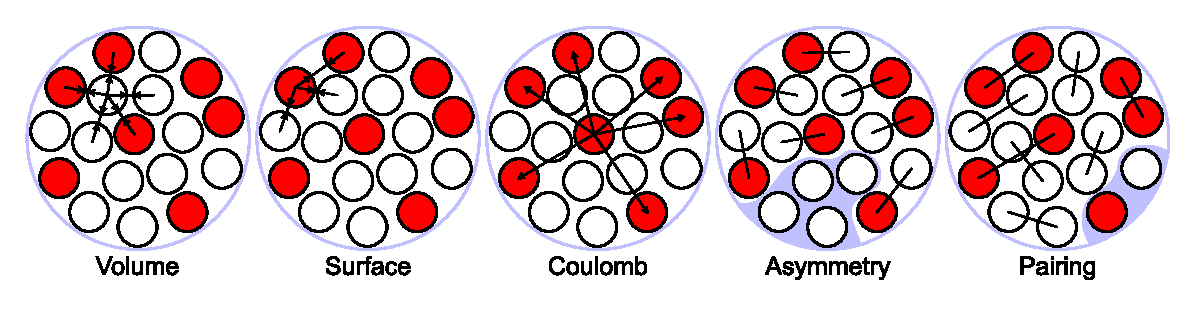
\includegraphics[width=1.0\textwidth]{Images/Liquid_drop_model.pdf}
    \caption{Visual representation of the liquid drop model from \cite{ldmimg}}
    \label{fig:liquid_drop_model}
\end{figure}
The SEMF can be fitted on current data to get a good estimate of binding energies \cite{Benzaid2020}, but it still lacks the ability of describing many aspects of nuclear structure, mainly, the nuclear shell structure, which can account for magic numbers and nuclear deformations.
\subsection{Shell corrections}
Describing the nucleus through a shell model would account for the quantum mechanical nature of the system, unfortunately, unlike the `atomic' case, we don't have a source of the field to which nucleons are sucjected to, since it's generated by the nucleons themselves; nonetheless, the formulation of an empirical potential which reproduces experimental data has been proven to be successful in providing useful corrections to the liquid drop model.
\\The so called Woods-Saxon potential is an empirical field used for modelling the average field to which an independent nucleon would feel in a nucleus. It can take different parametrizations depending on the data that one wants to reproduce. It is formulated as to follow the shape of the nuclear density \eqref{eq:phen_density}, and it reads
\begin{equation}
    \label{eq:sphWS}
    U(\bm r) = -\frac{U_0(A, N)}{1+e^\frac{r - R}{a}}
\end{equation}
where $U_0$ is the potential depth
\begin{equation}
    U_0(A, N) = U_0\bigg(1\pm \kappa \frac{2N -A }A\bigg),
\end{equation}
the $+$ and $-$ signs refer to protons and neutrons respectively. $R$ refers to the radius of the nuclear surface, generally parametrized as 
\begin{equation}
    R=r_0 A^{1/3}
\end{equation}
and $a$ is the surface diffuseness, as in the density expression \eqref{eq:phen_density}.
\paragraph{Spin-orbit coupling} 
The success of the shell model is mainly due to the possibility of accounting for spin-orbit coupling, which is included through a term that reads
\begin{equation}
    U_{\text{LS}}(\bm r )=U_0^{\text{LS}}\bigg(\frac{r_0}{\hbar}\bigg)^2 \frac 1 r \dv{}{r}\bigg (\frac{1}{1+e^{\frac{r-R}{a}}}\bigg).
\end{equation}
\paragraph{Coulomb interaction}
In the spherical case, the coulomb interaction can be taken as the energy potential produced by a sphere of charge $Z$ and radius $R$, which reads
\begin{equation}
    U_{\text{C}}(r) = Ze^2
    \begin{cases}
        \frac{3-(r/R)^2}{2R} & r \le R, \\
        \frac 1 r & r > R.
    \end{cases}
\end{equation}
The complete Hamiltonian then reads
\begin{equation}
    \hat H = \hat T + U + U_{\text{LS}}+U_C,
\end{equation}
where $U_C$ is present only when solving for the proton shells. The solution to the eigenvalue problem $\hat H \psi = E\psi$ is of the form
\begin{equation}
   \psi_{nljm_j} = \frac{u_{nl}(r)}{r}[Y_{l}(\hat {\bm r})\otimes \chi_{1/2}]_{jm_j} 
\end{equation}
where $Y_{nl}(\hat {\bm r})$ is the spherical harmonic function of degree $l$ and order $m$, the $\hat r$ is used to denote dependence on the azimuthal and polar angles of $\bm r$ and $\otimes$ takes the meaning of the angular momentum coupling and $u_{nl}(r)$ satisfies the reduced Schr\"odinger equation
\begin{equation}
    \label{eq:red}
    \bigg(-\frac {\hbar^2}{2m}\dv[2]{r}+\frac{\hbar l(l+1)}{2mr^2}+U(r)\bigg)\psi_{nl} = E\psi_{nl}.
\end{equation}
The effect of the spin-orbit coupling $U_{\text{LS}}$ and the Coulomb repulsion $U_C$ can be accounted for by using first order perturbation theory.
\subsubsection{Harmonic oscillator}
A small digression on the harmonic oscillator is in order. The solution of the spherical potential 
\begin{equation}
U_{\text{HO}} (\bm r ) = \frac 1 2 m\omega^2 r^ 2,
\end{equation}
produces the spherical harmonic oscillator basis, which is very similar to the basis one would get solving for the Woods-Saxon potential, provided that $\omega$ is taken as $41/A^{1/3}$ MeV. As a matter of fact, the harmonic oscillator basis is often used to perform calculations in nuclear physics. We will see in section \ref{sec:minimization} that a harmonic oscillator basis is used as starting guess for the numerical solution of a Woods-Saxon potential.
\subsubsection{Shell structure}
A graphical representation of the shells for a harmonic oscillator is shown in figure \ref{fig:shell_model}, where the contribution of the spin-orbit coupling is also accounted for; unlike the atomic case, shells whose total angular momentum is higher are lowered in energy, viceversa for lower total angular momentum.  
\begin{figure}[h]
    \centering
    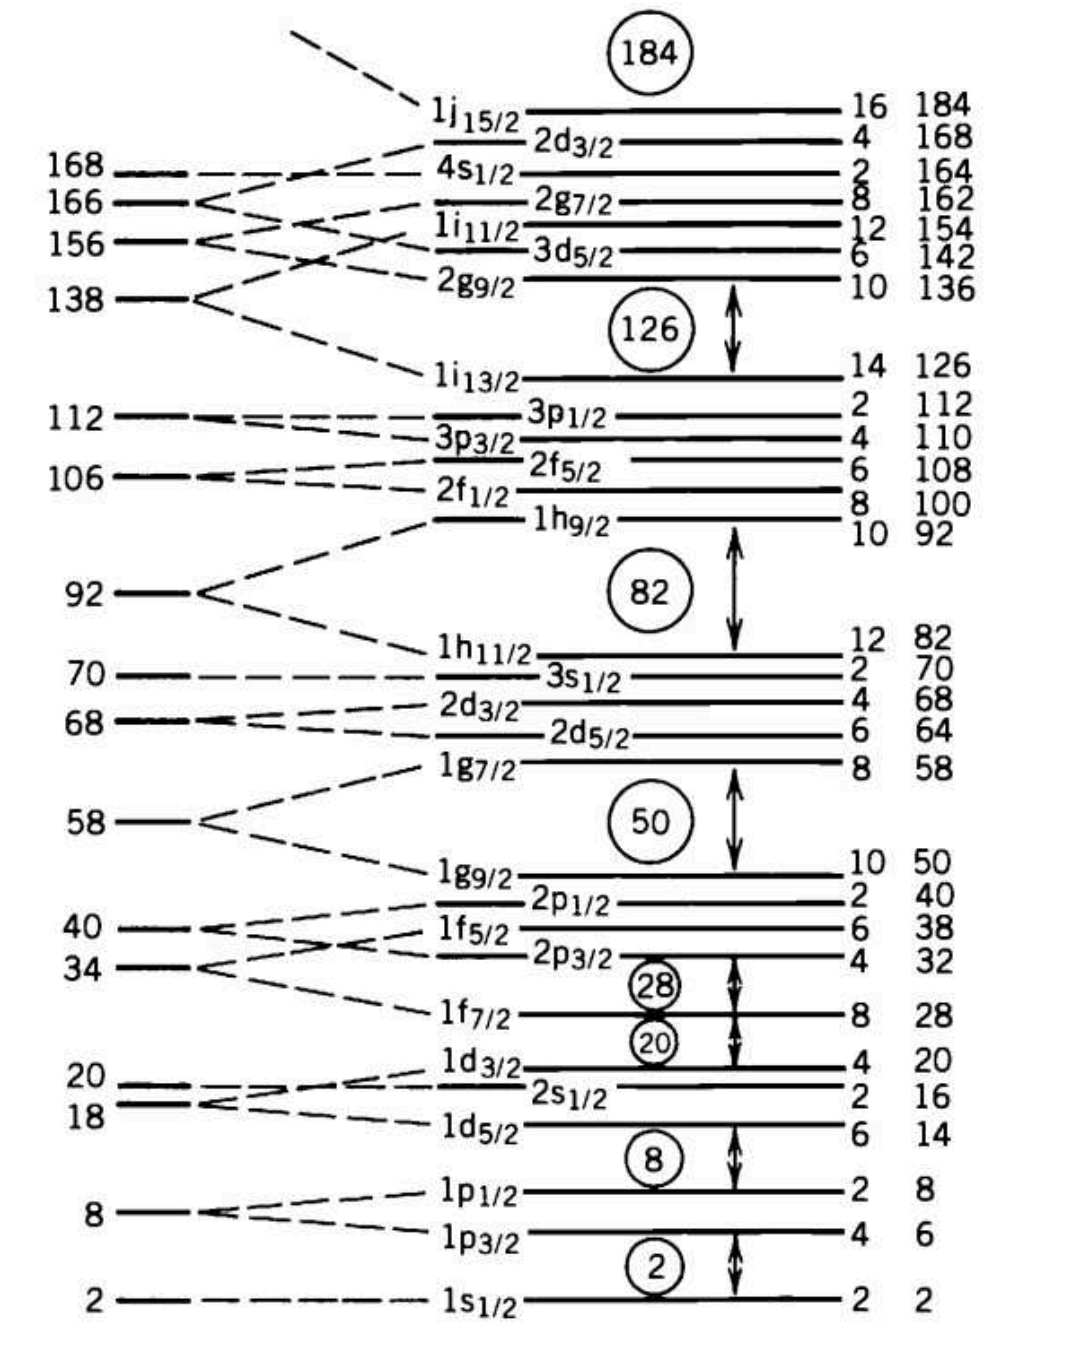
\includegraphics[width=0.5\textwidth]{Images/ShellModel.png}
    \caption{Graphical representation of a harmonic oscillator shells, together with the spin-orbit coupling. Shells whose total angular momentum is higher are lowered in energy, viceversa for lower total angular momentum.}
    \label{fig:shell_model}
\end{figure}



\section{Nuclear pairing}
\label{sec:pairing_intro}
In the semi-empirical mass formula \eqref{eq:semf}, the $\delta_p$ term can be parametrised as 
\begin{equation}
    \delta_p = \begin{cases}
        +\delta_0 & \text{ if N and Z are even}, \\
        0 & \text{ if A is odd}, \\
        -\delta_0 & \text{ if N and Z are odd},
    \end{cases}
\end{equation}
hence having an even number of neutrons and/or protons increases the binding energy of the nucleus. A common choice for $\delta_0$ is
\begin{equation*}
\delta_0 = 12 A^{1/2}\text{ MeV}.
\end{equation*}
This is a phenomena closely related to superconductivity, as nucleons of the same type form pairs that lie in higher energy states. An experimental evidence of this fact is knwon as odd-even staggering, where the separation energy
\begin{equation}
    S_n = E_B(A, Z) - E_B(A-1, Z),
\end{equation}
is higher for even $A$, an increase that corresponds to the energy necessary to break a pair. We will see in section \ref{sec:pairing_hf} the two main methods to account for pairing at a microsopic level.



\section{Nuclear deformations}
\label{sec:deformations}
We shall now give a description of the nuclear shape in a formal framework. We will start by expanding the nuclear radius in terms of spherical harmonics, so that we can truncate and omit terms to describe certain configurations of the nucleus, so that we are able to illustrate the simple case of an axial quadrupole deformation. After that, we will briefly discuss the more general case of trixial, octupole, and parity breaking configurations.
\subsection{Quadrupole deformation}
Assuming the nuclear volume to be evaluated as
\begin{equation}
    \label{eq:volume}
    V(A) = \frac{4}{3}\pi R^3
\end{equation}
Let us suppose to consider variations of the nuclear radius $R$ in terms of spherical harmonics
\begin{equation}
    R(\theta, \phi) = R_0\bigg[1+\sum_{\lambda \mu}\alpha_{\lambda \mu}\,Y_{\lambda\mu}(\theta,\phi)\bigg]
\end{equation}
where the moments $\alpha_{\lambda \mu}$ defined as
\begin{equation}
    \alpha_{\lambda \mu}=\int Y_{\lambda\mu}^*(\theta, \phi)R(\theta, \phi) d\Omega,
\end{equation}
are considered small, in the sense that $|\alpha_{\lambda \mu}| ^2 \ll |\alpha_{\lambda \mu}| $ as to conserve the volume in equation \eqref{eq:volume}. We have that $Y_{00}$ is constant, so its moment does not provide additional information to the constant radius. We can set $\alpha_{00}=0$. 
Since $Y_{10}$, $Y_{11}$ and $Y_{1-1}$ are odd for $\theta + \pi$ and $\phi + \pi$, we have that $\alpha_{1\mu}$ vanishes in a reference frame in which the centre of mass is at the origin.
\\Now, let us consider only $\alpha_{2\mu}$ coefficients and neglect higher degree terms, so that the deformation is purely quadrupolar, then the radius reads
\begin{equation}
    R(\theta, \phi) = R_0\bigg[1+\sum_{\mu=-2}^2\alpha_{2\mu}\,Y_{2\mu}(\theta, \phi)\bigg].
\end{equation}
If we assume to be in the reference frame in which the inertia tensor, proportional to the coefficients $\alpha_{2\mu}$, is diagonal, which is known as intrinsic frame, then the sum 
\begin{equation*}\alpha_{21}Y^*_{21} + \alpha_{2-1}Y^*_{2-1}\end{equation*} vanishes. Since $R$ is a real valued function, we have the relation
\begin{equation}
\alpha_{\lambda \mu}Y_{\lambda\mu}+\alpha_{\lambda -\mu}Y_{\lambda-\mu}=2\Re{\alpha_{\lambda \mu}Y_{\lambda\mu}},
\end{equation}
as a consequence, the resulting expansion reads
\begin{align}
    R(\theta, \phi) &= R_0\bigg[1+a_{20}Y_{20}+2\Re{a_{22}Y_{22}}\bigg]\nonumber
    \\&=R_0\bigg[1+\sqrt{\frac{5}{16\pi}}\bigg(a_{20}(3\cos^2\theta-1)+ 2a_{22}\sqrt{3}\sin^2\theta(\cos^2\phi-\sin^2\phi) \bigg)\bigg].
\end{align}
If we perform the substitution 
\begin{align}
    \label{eq:a20}
    a_{20} &= \beta\cos(\gamma)
    \\  a_{22} &= \beta\sin(\gamma)\label{eq:a22}
\end{align} 
and express the variation of $R$ along the cartesian axes, we get 
\begin{align}
     R_x - R_0  =\delta R_{x}&=\sqrt{\frac{5}{4\pi}}\beta R_0 \cos\bigg(\gamma - \frac{2\pi}{3}\bigg),
    \\R_y - R_0 =\delta R_{y}&=\sqrt{\frac{5}{4\pi}}\beta R_0 \cos\bigg(\gamma + \frac{2\pi}{3}\bigg),
    \\R_z - R_0 =\delta R_{z}&=\sqrt{\frac{5}{4\pi}}\beta R_0 \cos\gamma.
\end{align}
Assuming the value of $\beta$ to always be positive, in the case $\gamma=0$, $\delta R_x = \delta R_y <\delta R_z$, meaning the nucleus is in a \textit{prolate} configuration; while in the case of $\gamma = \pi/3$, $\delta R_x = \delta R_y > \delta R_z$, meaning the nucleus has an \textit{oblate} shape. A general convention is to write $\beta$ with a negative sign in the oblate case, and a positive sign in the prolate case.
\\By using trigonometric identities, it is trivial to show that unique shapes are found only for $\gamma\in [0; \pi/3]$, if $\gamma$ takes a value different from $0$ or $\pi/3$, the shape is said to be triaxial, meaning $\delta R_z \neq \delta R_x \neq \delta R_y$, the nucleus has no more rotational symmetries and is only symmetric for reflections along the $(x, y)$, $(x, z)$ and $(y, z)$ planes, which also induces parity symmetry.
\subsection{Nilsson model}
To understand the effect on single-particle motion of a deformed potential, we can consider the case of an axially deformed harmonic oscillator potential, for which $ \omega_z \neq \omega_x = \omega_y = \omega_\perp$, meaning the oscillator frequency takes on a different value on the $z$ axis than in the $x$ and $y$ axes.
\\To treat the deformation perturbatively, we can assume that the various frequencies deviate from the unperturbed $\omega_0=41/A^{1/3}$ MeV, in which case they may read
\begin{align}
\omega_z = \omega_0 - \frac 2 3 \varepsilon,\\
\omega_\perp = \omega_0 + \frac 1 3 \varepsilon,
\end{align}
this definition of the frequencies satisfies the conservation of volume, at lowest order in $\varepsilon$, assumed to hold for 
\begin{equation}
    \label{eq:volume_cons}
    \omega_0 ^ 3 = \omega_z \omega_\perp^2.
\end{equation}
We can thus write the single-particle Hamiltonian in the deformed potential as
\begin{align}
    H&=H_0 +\varepsilon H_1,\\
    H_0 &= -\frac{\hbar^2}{2m}\nabla^2 + \frac 1 2 m \omega_0^2 r^2,\\
    \varepsilon H_1 &= \frac 1 3 \omega_0 ^2 \varepsilon (x^2 + y^2 -2z^2) = -\frac 1 3 \sqrt{\frac{16\pi}{5}}m\omega_0^2\varepsilon r^2 Y_{20}.
\end{align}
$H_0$ is the usual spherical harmonic potential, for which the eigenfunctions, expressed through the usual quantum numbers $\ket{nljm_j}$ are known. Assuming $\varepsilon$ to be small, we can evaluate the first order correction of $H_1$ to the system, which reads
\begin{align}
\Delta E &= \bra{nljm_j}\varepsilon H_1 \ket{nljm_j},
\\&= -\frac 1 3 \sqrt{\frac{16 \pi}{5}}\varepsilon m \omega_0^2 \int r^2 u_{nl}(r)\bra{jm_j} Y_{20}\ket{jm_j} dr,
\\&= \frac \varepsilon 6 m\omega_0^2 \int r^2 u_{nl}(r)\frac{3m_j^2 - j(j+1)}{j(j+1)}dr,
\end{align}
thus in the limit of large $j$, states with the maximum total angular momentum projection $m_j$ are shifted upwards, while states with the minimum $m_j$ are shifted downwards; moreover, eigenstates with $\pm m_j$ are degenerate, as expected by the reflection symmetry of the Hamiltonian if the $z$ axis is inverted.
Adding further empirical terms to reproduce experimental data, and the spin-orbit coupling, results in the formulation of the Nilsson model \cite{nilsson}. In figure \ref{fig:nilsson}, a graphical representation of the energy levels in the Nilsson model is shown \cite{wikipedia_equation_of_state}.
\begin{figure}[h]
    \centering
    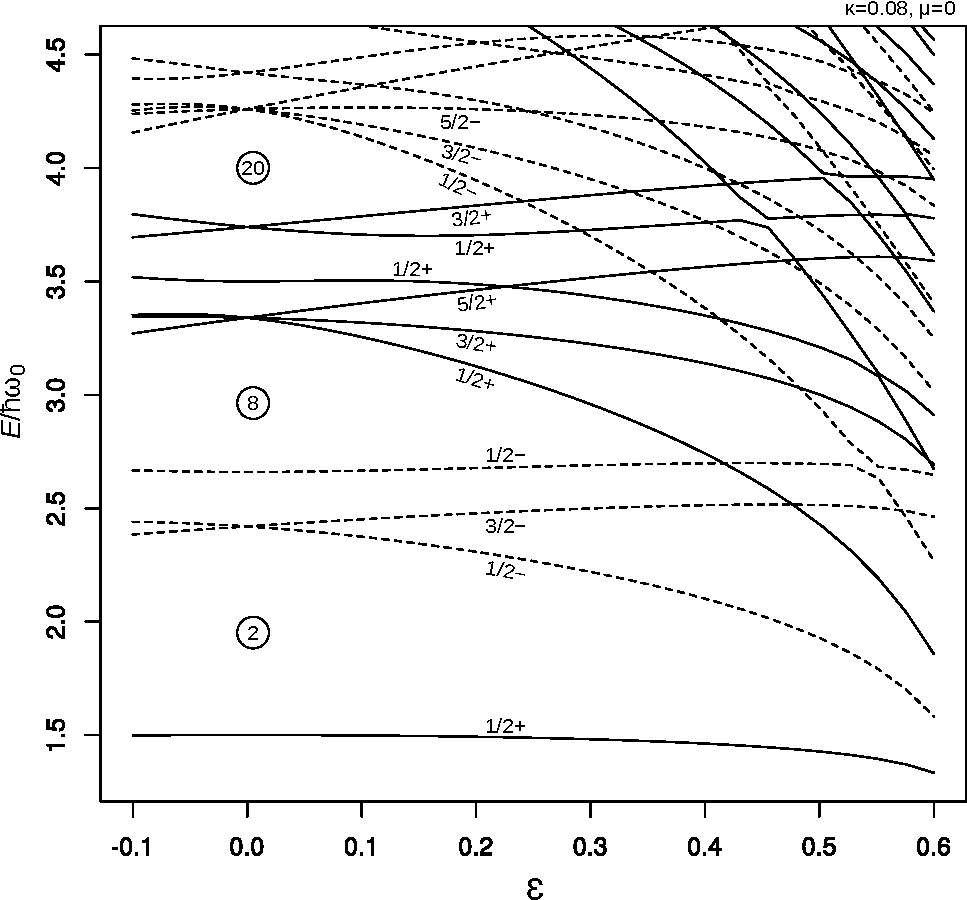
\includegraphics[width=0.7\textwidth]{Images/nilsson.pdf}
    \caption{Nilsson model energy levels trends, as a function of $\varepsilon$.}
    \label{fig:nilsson}
\end{figure}
\subsubsection{Deformed Woods-Saxon}
Recent studies of deformed nuclei have been carried out using empirical potentials such as deformed Woods-Saxon potentials \cite{def_WS_dudek,defWSfissionbarriers}. In these models, the nuclear shape is expanded as 
\begin{equation}
R(\theta) = R_0\bigg[1+\sum_{\lambda}^L \beta_{\lambda}Y_{\lambda 0}\bigg],
\end{equation}
so that the solution is axially symmetric and the problem is reduced to just the $(r, \theta)$ coordinates, in which we can write the potential as
\begin{equation}
    \label{eq:def_WS}
    U_\text{WS}(r, \theta) = -\frac{U_0(A, N)}{1+e^\frac{r - R(\theta)}{a}}.
\end{equation}
\subsection{Octupole deformations and parity breaking}
While quadrupole deformations concern nuclei across the whole chart, octupole deformations are much less common, being found only in heavier nuclei.
Under the parity operation $\mathcal P: \bm r \mapsto -\bm r$, coefficients of the spherical harmonics transform as
\begin{equation}
    \mathcal P \alpha_{\lambda \mu} = (-1)^{\lambda} \alpha_{\lambda \mu},
\end{equation}
hence a nuclear octpuole deformation, whose degree $\lambda=3$, would break parity symmetry. In figure \ref{fig:octupole_defs} a graphical representation of the spherical harmonics for $\lambda=3$ and $\mu=0,2$ is shown.
\begin{figure}[h]
    \centering
\begin{minipage}{0.48\textwidth}
    \centering
    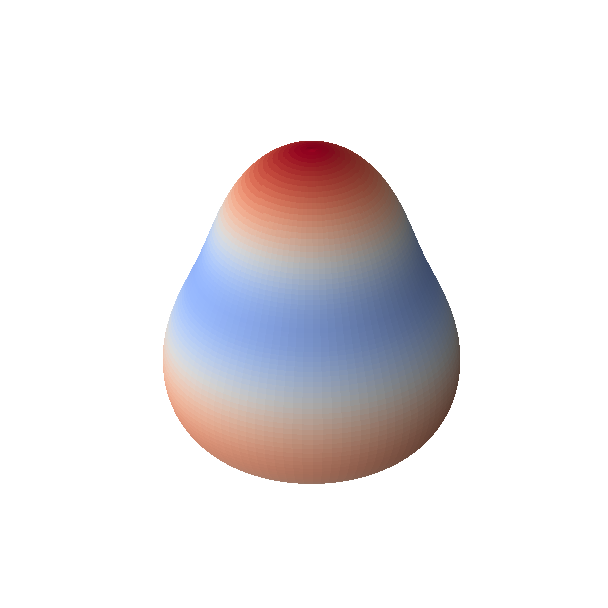
\includegraphics[width=\textwidth]{Images/octupole_Y30}
  \end{minipage}
  \hfill
  \begin{minipage}{0.48\textwidth}
    \centering
    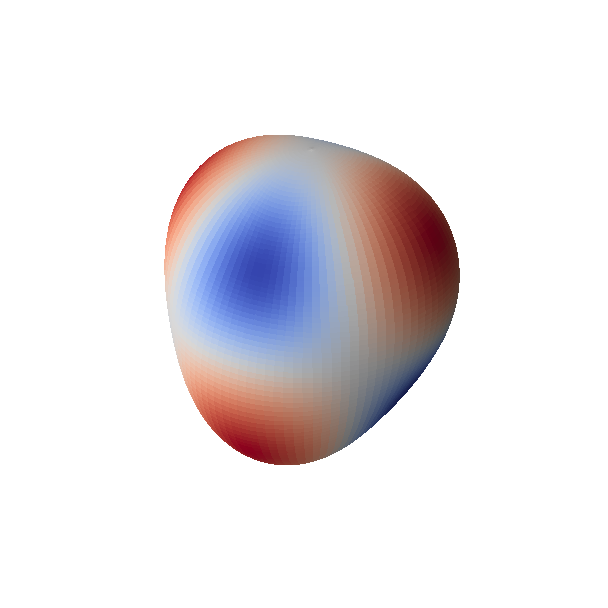
\includegraphics[width=\textwidth]{Images/octupole_Y32}
  \end{minipage}
    \caption{Graphical representation of possible octupole deformations. On the left, the axially symmetric $Y_{30}$ deformation, on the right, the non-axial octupole deformation $Y_{32}$.}
    \label{fig:octupole_defs}
\end{figure}





\section{Nuclear fission}
\label{sec:fission}
Nuclear fission is the process by which a nucleus splits into two -- sometimes three -- nuclei, whether spontaneously, or induced by a reaction.
The physics that governs nuclear fission is the one of many-body, large amplitude collective modes, which elongate the the nuclear shape, until the so called \textit{fission barrier} is surmounted and the path to the energy minimum is one where the nuclei fragments itself.
\subsubsection{Spontaneous fission model}
It should be ovious that a formal treatment of deformations and collective modes is necessary to give a theoretical description of fission reactions. We can derive a simple spontaneous fission model by studying the effect of a simple axial quadrupole deformation on the semiempirical mass formula \ref{eq:semf}.
\\Let us assume that the nuclear radius may be expanded, as previously done in section \ref{sec:deformations}, as
\begin{equation}
    R = R_0[1+\alpha_{20}Y_{20}].
\end{equation}
Assuming the nuclear volume is conserved across the fission path, the volume energy will not change. As for the surface energy, its variation can be expressed at the lowest order in $\alpha_{20}$ as
\begin{equation}
    \Delta E_\text{surf} = E_\text{surf}
    -E_{0,\text{surf}} = E_{0, \text{surf}}\frac 2 5 \alpha_{20}^2.
\end{equation}
Regarding the Coulomb energy, the variation is given by
\begin{equation}
    \Delta E_\text{coul} = E_\text{coul} - E_{0, \text{coul}} = -E_{0, \text{coul}}\frac 1 5 \alpha_{20}.
\end{equation}
Since the neutron and proton count does not change, the surface and Coulomb energies are the only contributions to the total energy difference. We can write
\begin{equation}
    \label{eq:fission_semf}
    \Delta E = \frac 2 5 \alpha_{20}^2 a_s A^{2/3}- \frac 1 5 \alpha_{20}^2 a_c Z^2 A^{-1/3},
\end{equation}
if we set equation \eqref{eq:fission_semf} to zero, we get, other than the undeformed solution for $\alpha_{20}=0$, 
\begin{equation}
    \frac{ Z^2}{A} = \frac{2 a_s}{a_c},
\end{equation}
where the ratio $2a_s/a_c$ amounts to $\approx 50$ in typical parametrizations of the SEMF. Equation \eqref{eq:fission_semf}, shows that for values of the so called \textit{fissility parameter} $Z^2/A$ larger than $50$, the energy change becomes negative, favouring a configuration in which the nucleus fragments due to the spontaneous fission.
\subsection{Octupole deformations}

\chapter{State of the art, objective and motivation}
\label{chap:methods}
\section{State of the art and motivation}
The need to account for nuclear deformations has been highlighted in chapter \ref{chap:intro}, particularly in regard to heavy nuclei and the fission process in section \ref{sec:fission}. The solution of the many-body problem has always been a computational challenge, mainly mitigated by using expansions on bases or assuming certain symmetries to reduce the dimensionality of the problem.
\\The problems that arise when using either of the aforementioned approaches call for the implementation of unconstrained codes.
\paragraph{Basis expansions} 
An efficient method to solve the many-body problem is to use basis expansions of the harmonic oscillator, similar to the nuclear system as mentioned in section \ref{sec:models}. Several implement this kind of procedure, one of which is used in the present work to benchmark our own implementation in section \ref{sec:hfbtho}. The main limitation of such approach is that weakly bound states and large deformations are not well represented, the former due fundamentally different asymptotic behaviours for $r\to \infty$, between the HO -- $e^{-r^2}$ -- and loosely bound or quasi-resonant states -- $e^{-r}$ \cite{Stoitsov2003_PRCC68_054312,Dobaczewski1996_PRCC53_2809}, while the latter needs a large number of HO shells to converge, leading to an exponential increase of the computational cost \cite{Marevic2022_CPC}.
\paragraph{Symmetry assumptions} 
Another approach to reduce the complexity of the procedure is to assume certain symmetries, as to reduce the dimensionality of the problem to save computational time. The main example of such codes is the spherical solution \cite{VauhBrinkOriginal,hfbcsqrpa} of the Hartree-Fock equations, but axially symmetric ones exist as well \cite{Pei2008_HFBAX}. The limitations of such codes are obvious, as they systematically prevent the representation of certain broken symmetries.
\paragraph{Unconstrained codes}
In recent years, codes that solve the Hartree-Fock or Hartree-Fock-Bogoliubov problem on an unconstrained 3D mesh have been developed \cite{Ryssens2015_EV8,Ryssens2016_MOCCa,Maruhn2014_Sky3D,Chen2022_HFBFFT}. These codes are able to represent broken symmetries, but they require a huge amount of computational power to be run at an acceptable accuracy, unless certain assumptions are made, such as plane reflection \cite{Ryssens2015_EV8,Ryssens2016_MOCCa}.
Hence, the need to explore new, more computationally efficient methods to solve the many-body problem, as done in this thesis through the use of the General Conjugate Gradient method, detailed in section \ref{sec:gcg}.
\section{Objectives}
The aim of this work is to develop a new implementation of the Hartree-Fock method on an unconstrained 3D mesh, by the use of the General Conjugate Gradient method. The goals addressed by this work are the following:
\begin{itemize}
    \item assess the feasibility of the General Conjugate Gradient for the solution of large-scale eigenvalue problems;
    \item solve the self-consistent Hartree-Fock equations on an unconstrained 3D mesh;
    \item verify the numerical accuracy of the new implementation against existing spherical codes;
    \item gauge the numerical accuracy of deformations, comparing results with well established deformed codes; and
    \item attempt to produce novel results that specifically require an unconstrained implementaiton of this kind, and establish the advance brought to the field by this work.
\end{itemize}
\section{Methods}
The methods used in this work are the following:
\paragraph{Skyrme energy functional} The many-body problem is treated within the well established Hartree-Fock framework, detailed in section \ref{sec:hf}; as mentioned in the introduction in chapter \ref{chap:intro}, it is not sufficient, as a more general energy density functional approach has to be taken, which is developed in section \ref{sec:skyrme} for the Skyrme functional used in this work.
\paragraph{Finite differences and General Conjugate Gradient} After the main equations to be solved have been derived, the numerical methods used to solve them are detailed in chapter \ref{chap:numerical}, starting with the numerical discretization of the equations in section \ref{sec:finite_diff} and then solving the eigenvalue problem using an implementation of the General Conjugate Gradient method in section \ref{sec:gcg}. Finally closing with some remarks about specific details about the code and the algorithm parameters in section \ref{sec:minimization}.



\chapter{Energy functional}
\label{chap:hf}
\section{Hartree-Fock theory}
An empirical description of nuclear structure can be carried out using phenomenological models, as reported in section (REF).
\\A more rigorous approach needs to take into account the fact that the mean field which the nucleons interact with, is generated by the nucleons themselves, due to some microscopic interaction.
\\The many-body hamiltonian of the system, given by
\begin{equation}
    \label{eq:mb_hamiltonian}
    \hat H = \hat T + \hat V = \sum_i -\frac{\hbar^2}{2m}\nabla^2_i + \sum_{i<j} v^{(2)}_{ij} + \sum_{i<j<k} v^{(3)}_{ijk }
\end{equation}
acts on the nucleus, a system of $A$ nucleons described by the Slater determinant
\begin{equation}
    \label{eq:slater_formula}
    \Psi = \frac{1}{\sqrt {A!}} \sum_{\{p\}} (-1)^{p}  \varphi_{p(1)}(\bm r_1)\ldots \varphi_{p(A)}(\bm r_A)
\end{equation}
That is, summing over all possible permutations of the $A$ fermions on the single particle states, with a $-$ sign according to the parity of the permutation.
\subsection{Variational principle}
It is possible to show \cite{ring2004nuclear} that the ground state of the many-body system, found by minimizing the functional
\begin{equation}
    \label{eq:functional_hf}
    E[\Psi] = \frac{\bra{\Psi} \hat H \ket{\Psi}}{\bra{\Psi} \ket{\Psi}}
\end{equation}
Is equivalent to the 




\section{Functional}


\section{Pairing in Hartree-Fock theory}
\label{sec:pairing_hf}
In this section, we will discuss the two common approaches to include nuclear pairing in the HF theory. The aim of these few pages is to provide a brief overview of how the BCS equations are derived and understand the basics of the more general Hartree-Fock-Bogoliubov theory. The former method is the most widely implemented thanks to its low complexity \cite{hfbcsqrpa,oldEv8,skyax}, while the latter, more sophisticated and advanced, is the standard in modern codes \cite{hfodd, hfbftt,MAREVIC2022108367}. We will touch on it so that the reader may appreciate in the numerical chapter the natural extension of this work to the more general Bogoliubov ansatz. 
\subsection{BCS theory}
The BCS approximation, from Bardeen-Cooper-Schrieffer, is the same theory used to describe Cooper pairs in superconductivity, applied to the nuclear case.
The ansatz of BCS is that nucleons are paired in states whose total angular momentum is zero, such a wavefunction can be expressed as $\ket{JM}=\ket{00}$ and reads
\begin{equation}
    \label{eq:zero_mom}
    \ket{00} = \sum_{m_j} \bra{jm_j j-m_j}\ket{00}\ket{jm_j}\ket{j-m_j}
\end{equation}
Introducing the time-reversal operator $\hat {\mathcal T}:t\mapsto -t$, it acts on $\ket{00}$ as 
\begin{equation}
    \hat {\mathcal T} \ket{jm_j} = \widetilde{\ket{{jm_j}}} = (-1)^{j+m_j}\ket{j-m_j},
\end{equation}
using this relation, equation \eqref{eq:zero_mom} becomes 
\begin{equation}
    \ket{00} =- \frac{1}{\sqrt{2j+1}}\sum_{m_j}\ket{jm_j}\widetilde{\ket{{jm_j}}}.
\end{equation}
Hence BCS amounts to replacing the Slater determinant with a more general wavefunction to describe the ground state, which reads
\begin{equation}
    \label{eq:bcs_det}
    \bcs = \prod_{k>0}(u_k+ v_k a_{\tilde k}^\dagger a_k^\dagger) \ket{-}
\end{equation}
where $u_k$ and $v_k$ are real parameters whose meaning will shortly be clear, $k$ is short-hand for $\ket{jm}$, and $\tilde k = -k$ denotes the time-reversal state of $k$; the product runs over positive $k$ only. The BCS wavefunction is the creation in the vacuum of quasi-particles made of time-reversal paired particles, instead of individual ones. The normalization condition on the BCS wavefunction reads
\begin{equation}
    \label{eq:bcs_norm}
    1=\braket{\text{BCS}} = \prod_{k>0} \bra{-}(u_{k}+v_{k}a_{k}a_{\tilde k})(u_k+v_k a_{\tilde k}^\dagger a_k^\dagger)\ket{-} =\prod_{k>0}(u_k^2+v_k^2)=1
\end{equation}
which implies, for every pair $k$, the condition
\begin{equation}
    \label{eq:norm_uv}
    u_k^2+v_k^2=1.
\end{equation}
Taking the expectation value of the particle number operator $\hat N = \sum_k a_k ^\dagger a_k$ yields \cite{bertulani2007nuclear}
\begin{equation}
    \bbcs \hat N \bcs = 2\sum_ {k>0} v_k^2,
\end{equation}
while the expectation value of the particle number dispersion reads
\begin{equation}
\expval{\Delta\hat N ^2} = \expval{\hat N^2} - \expval{\hat N}^2 = 4\sum_{k>0} v_k^2 u_k^2.
\end{equation}
The consequence of this result is profound. The BCS ansatz does not assume a fixed number of particles, rather it becomes an observable of the system, with an expectation value that depends on how the parameters $v_k^2$ are set, which represent the probability of finding a particle in the $k$-th state.
We can now write the many body Hamiltonian of the system as in equation \eqref{eq:mb_hamiltonian_sq}
\begin{equation}
    \hat H = \sum_{k_1 k_2}t_{k_1k_2} a_{k_1}^\dagger a_{k_2} + \frac 1 4 \sum_{k_1 k_2 k_3 k_4}\overline{v}_{k_1k_2k_3k_4} a_{k_1}^\dagger a_{k_2}^\dagger a_{k_3} a_{k_4}
\end{equation}
and replace it with the Routhian 
\begin{equation}
    \label{eq:bcs_routhian}
    \bbcs \hat H - \lambda \hat N \bcs
\end{equation}
so that the expected number of particles may be fixed, under the appropriate choice of $\lambda$, by the relation
\begin{equation}
\pdv{}{N}\bbcs \hat H  \bcs = \lambda.
\end{equation}
the Lagrange multiplier $\lambda$ takes on the meaning of the Fermi energy.
We can now apply the variational principle \eqref{eq:var_eq_res} to \eqref{eq:bcs_routhian} using the $v_k$ as variational quantities, which yields 
\begin{equation}
   4\tilde \varepsilon_k ^2 u_k^2 v_k^2 = \Delta_k ^2 - 4\Delta_k^2 u_k^2v_k^2,
\end{equation}
where the pairing gap $\Delta_k$ is defined as
\begin{equation}
    \label{eq:delta_k}
    \Delta_k = - \sum_{k'}\overline v_{k\tilde k k'\tilde{k'}}v_{k'}u_{k'} 
    \end{equation}
and the quantity $\tilde\varepsilon_k$ is defined as 
\begin{align}
    \label{eq:epsilon}
    \tilde \varepsilon_k &= \frac 1 2 \bigg[t_{kk} + t_{\tilde k \tilde k }-2\lambda +\sum_{k'}(\overline v_{k\tilde k k'\tilde{k'}}v_{k'}u_{k'} + \overline v_{\tilde k k' \tilde k k'})v_{k'}^2\bigg]
    \\&=\frac 1 2 [h_{kk}+h_{\tilde k \tilde k}]-\lambda.
\end{align}
Introducing the quasi-particle energy
\begin{equation}
    \label{eq:qpe}
    E_k = \sqrt{\tilde \varepsilon_k^2 +\Delta_k^2}
\end{equation}
we can combine definitions \eqref{eq:delta_k} and \eqref{eq:qpe} with equation \eqref{eq:epsilon}, under the normalization condition \eqref{eq:norm_uv}, to get an equation for $v_k^2$
\begin{equation}
    \label{eq:v2}
    v_k^2 = \frac 1 2 \pm \frac{|\tilde \varepsilon_k|}{2E_k}.
\end{equation}
Since in the Hartree-Fock limit, where the occupations $v_k^2$ are equal to one below the fermi energy and zero above, and the gaps $\Delta_k$ vanish, rendering $E_k=\tilde \varepsilon_k$, we only select the solution
\begin{equation}
v_k^2 = \frac 1 2 - \frac{\tilde \varepsilon_k}{2E_k}.
\end{equation}
Using the normalization condition to write $u_k^2=1-v_k^2$, and plugging it into the gaps definition \eqref{eq:delta_k}, we arrive to the gap equation
\begin{equation}
    \label{eq:gap}
    \Delta_k = - \sum_{k'}\frac{\Delta_{k'}\overline v_{k\tilde k k'\tilde{k'}}}{2E_{k'}}
\end{equation}
The system of equations (\ref{eq:gap}, \ref{eq:norm_uv}, \ref{eq:v2}, \ref{eq:qpe}, \ref{eq:epsilon}), together with the condition on $\hat N$ -- ie $\expval{\hat N}=N$ -- is closed and can be solved numerically, usually through an effective pairing interaction.
\subsection{Hartree-Fock-Bogoliubov theory}
\label{sec:hfb}
The most general ansatz to account for pairing interactions in Hartree-Fock theory is the Hartree-Fock-Bogoliubov (HFB) theory, it allows a treatment of the mean-field and pairing interactions in a unified way, the quasi-particles created on the vacuum are the most general ones, instead of being time-reversal paired particles.
Let us start by writing a Bogoliubov transformation from the particle basis $c_i$ to a quasi-particle one 
\begin{equation}
    \label{eq:bogoliubov_trans}
    \beta_k^\dagger = \sum_l U_{lk} c_l^\dagger + V_{lk} c_l.
\end{equation}
If we take the Hermitian conjugate of the relation \eqref{eq:bogoliubov_trans}, we get the transformation for $\beta_k$, we are then able to write in matrix form
\begin{equation}
    \label{eq:bogoliubov_trans_mat}
    \begin{pmatrix}
    \beta\\
    \beta^\dagger
    \end{pmatrix}
    =\begin{pmatrix}
        U^\dagger & V^\dagger \\
        V^T & U^T
    \end{pmatrix}
    \begin{pmatrix}
        c\\
        c^\dagger
    \end{pmatrix}
    =\mathcal W^\dagger \begin{pmatrix}
        c\\
        c^\dagger
    \end{pmatrix},
\end{equation}
where the matrix of matrices $\mathcal W$ reads
\begin{equation}
    \label{eq:bogoliubov_mat}
    \mathcal W = \begin{pmatrix}
        U & V^*\\
        V & U^*
    \end{pmatrix}.
\end{equation}
Taking the product $\mathcal W^\dagger \mathcal W$ and imposing separate fermionic commutation relations of the operators $\beta, \beta^\dagger, c, c^\dagger$, we get that $\mathcal W$ is unitary, hence
\begin{equation}
    \mathcal W^\dagger \mathcal W = \mathcal W \mathcal W^\dagger =  I.
\end{equation}
We can now invert equation \eqref{eq:bogoliubov_trans_mat} by multiplying both sides on the left by $\mathcal W$, which yields 
\begin{equation*}
    \mathcal W \begin{pmatrix}
        \beta\\
        \beta^\dagger
    \end{pmatrix}
    =\begin{pmatrix}
        c\\
        c^\dagger
    \end{pmatrix}.
\end{equation*}
Using the Messiah-Bloch decomposition \cite{blochmessiah}, we can write the unitary matrix $\mathcal W$ as
\begin{equation}
    \label{eq:decomposition}
    \mathcal W = \begin{pmatrix}
        D & 0 \\
        0 & D^*
    \end{pmatrix}
    \begin{pmatrix}
        \overline U & \overline V \\
        \overline V & \overline U
    \end{pmatrix}
    \begin{pmatrix}
        C & 0 \\
        0 & C^*
    \end{pmatrix}
\end{equation}
where $D$ and $C$ are unitary matrices and $\overline U$ and $\overline V$ are real matrices, which have a particular blocked form, expressed through the coefficents $u_k, v_k$; the reader may refer to appendix \ref{app:uv} for the explicit representation. We can also define the matrices $U, V$ as 
\begin{equation}
    U=D\overline U C,\quad V=D^*\overline V C.
\end{equation}
Using the decomposition \eqref{eq:decomposition} we can define the \textit{canonical basis} as
\begin{equation}
    \label{eq:canonical_basis}
    a_k^\dagger = \sum_l D_{lk}^\dagger c_l^\dagger,
\end{equation}
a \textit{special Bogoliubov transformation} between \textit{paired} levels as
\begin{align}
    \alpha_k^\dagger = u_k a_k^\dagger - v_k a_{\tilde k},\\
    \alpha_{\tilde k } ^\dagger = u_k a_{\tilde k} ^\dagger + v_k a_k,
\end{align}
and \textit{blocked} levels
\begin{align}
\alpha_i &= a_i,\quad \alpha_n^\dagger = a_n^\dagger
\\\alpha_i &= a_i^\dagger, \quad \alpha_n = a_n,
\end{align}
where $u_k=u_{\tilde k},\ v_k=-v_{\tilde k}$, and a unitary transformation of the quasi-particle operators $\alpha_k^\dagger$ among themselves
\begin{equation}
    \beta_k^ \dagger = \sum_{k'}C_{k'k}a_{k'}^\dagger.
\end{equation}
We are now able to define the Bogoliubov ground state $\ket{\text{HFB}}$, as the one for which
\begin{equation}
    \beta_k \ket{\text{HFB}} = 0 \ \forall k = 1,\ldots,M
\end{equation}
where $M$ is determined by the physical situation \cite{ring2004nuclear}.
The wavefunction that satisfies this condition reads
\begin{equation}
\ket{\text{HFB}}=\prod_k^M\beta_k \ket{-}.
\end{equation}
We can define the pairing tensor as
\begin{equation}
    \kappa_{ll'} = \bra{\text{HFB}}c_{l'}c_l\ket{\text{HFB}},
\end{equation}
which in matrix form reads, alongside the density matrix
\begin{equation}
    \kappa = UV^\dagger,\quad \rho = V^*V^T.
\end{equation}
We can now apply the variational principle \eqref{eq:var_eq_res}
\begin{equation}
    \label{eq:varhfb}
    \delta \frac{\bra{\text{HFB}} \hat H-\lambda \hat N\ket{\text{HFB}}}{\bra{\text{HFB}}\ket{\text{HFB}}} = 0.
\end{equation}
which yields the eigenvalue problem
\begin{equation}
    \label{eq:eighfb}
    \begin{pmatrix}
    h -\lambda& \Delta \\ -\Delta^* & -(h-\lambda)^*
    \end{pmatrix}
    \begin{pmatrix}
        U_k \\ V_k
    \end{pmatrix}
    =\mathcal H_\text{HFB}\begin{pmatrix}U_k \\V_k\end{pmatrix}= E_k \begin{pmatrix}
        U_k \\ V_k
    \end{pmatrix},
\end{equation}
Here, $h$ is the single-particle Hamiltanian, which reads
\begin{equation}
    h_{kk'} = t_{kk'} +\Gamma_{kk'},
\end{equation}
where $\Gamma_{kk'}$ is the mean field potential, given by
\begin{equation}
    \label{eq:mean_field_hfb}
    \Gamma_{kk'} = \sum_{ll'}\overline{v}_{kl'k'l}\rho_{ll'}
    \end{equation}
and the pairing field $\Delta$ reads
\begin{equation}
    \label{eq:pairing_field_hfb}
    \Delta_{kk'} = \sum_{ll'}\overline{v}_{kk'll'}\kappa_{ll'}.
\end{equation}
In the canonical basis, we are able to solve for the occupation numbers
\begin{equation}
    \label{eq:occ_hfb}
    u_k^2 = \frac 1 2 \bigg(1+\frac{h_{kk}+h_{\tilde k \tilde k}}{\sqrt{(h_{kk}+h_{\tilde k \tilde k})^2+4\Delta_{k\tilde k}^2}}\bigg)
\end{equation}
where $v_k^2 = 1 - u_k^2$ is guaranteed by the unitarity of the matrices.
Starting from an initial guess, we solve the eigenvalue problem \eqref{eq:eighfb}, we extract the occupation numbers \eqref{eq:occ_hfb}, use them to build the new mean field \eqref{eq:mean_field_hfb} and pairing field \eqref{eq:pairing_field_hfb}, and repeat the process until convergence.
\paragraph{HFB quasi-particle spectrum} Let us assume that $\Psi = (U,\  V )^T$ is a solution of equation \eqref{eq:eighfb} with eigenvalue $E$
\begin{equation}
    \label{eq:eigsolhfb}
    \mathcal H_\text{HFB}\Psi = E\Psi.
\end{equation}
Let the particle-hole matrix $\mathcal C$ be defined as
\begin{align}
    \mathcal C = \begin{pmatrix}
        0 & I \\ I&0
    \end{pmatrix},
\end{align}
it's trivial to show that 
\begin{equation}
    \label{eq:hfb_anticomm}
    \mathcal C \mathcal H_\text{HFB} \mathcal C = -\mathcal H_\text{HFB}^*,
\end{equation}
and 
\begin{equation}
    \label{eq:commutationhfb}
    \mathcal C = \mathcal C ^{-1}\implies \mathcal C\mathcal H_\text{HFB} = -\mathcal H_\text{HFB}^*\mathcal C.
\end{equation}
If we take the complex conjugate of equation \eqref{eq:eigsolhfb}, we get
\begin{equation}
    \label{eq:eigsolhfb_conj}
    \mathcal H_\text{HFB}^*\Psi ^* = E\Psi^*,
\end{equation}
if we multiply both sides on the left by $\mathcal C$ and use \eqref{eq:commutationhfb}, we get
\begin{align}
    -\mathcal H_\text{HFB}\mathcal C\Psi ^* &= E\mathcal C\Psi^*,\\
    \mathcal H_\text{HFB}\mathcal C\Psi ^* &= -E\mathcal C\Psi^*,
\end{align}
meaning that $\mathcal C \Psi^*$ is a solution of the eigenvalue problem \eqref{eq:eighfb} as well, with eigenvalue $-E$, hence for every quasi-particle energy we have a corresponding opposite-sign one; moreover, it can be proven that the HFB hamiltonian is unbounded, both from below and above \cite{Pei2012_HFBcontinuum}. This feature poses a challenge for numerical solutions of the HFB problem, as we shall see in chapter \ref{chap:numerical}.




\section{Skyrme force and functional}
Now that the theoretical and numerical framework is clear, we can investigate a plausible nucleonic interaction, which in the present work, takes the form of the Skyrme interaction.
\\It was first proposed by Tony Skyrme in 1958 \cite{SKYRME1958615} as a zero range force between nucleons, and has been used successfully as the building block of nuclear structure.
\\Nowadays, the standard form is slightly enriched to be more general \cite{CHABANAT1997710}. It comprises a two-body interaction, which reads
\begin{align}
v^{(2)}(\mathbf{r}_1, \mathbf{r}_2) &= t_0 \left(1 + x_0 P_\sigma \right) \delta(\mathbf{r}) \\
&\quad + \frac{1}{2} t_1 \left(1 + x_1 P_\sigma \right) \left[ \mathbf{P}'^2 \delta(\mathbf{r}) + \delta(\mathbf{r}) \mathbf{P}^2 \right] \\
&\quad + t_2 \left(1 + x_2 P_\sigma \right) \mathbf{P}' \cdot \delta(\mathbf{r}) \mathbf{P} \\
&\quad + \frac{1}{6} t_3 \left(1 + x_3 P_\sigma \right) \left[ \rho(\mathbf{R}) \right]^\sigma \delta(\mathbf{r}) \\
&\quad + i W_0 \boldsymbol{\sigma}\cdot \left[ \mathbf{P}' \times \delta(\mathbf{r}) \mathbf{P} \right]
\end{align}
And a three body interaction, that is
\begin{equation}
v^{(3)}(\mathbf r_1, \mathbf r_2)=\frac 1 6 t_3 \left(1 + x_3 P_\sigma \right) \left[ \rho(\mathbf{R}) \right]^\sigma \delta(\mathbf{r}) 
\end{equation}
Where 
\begin{align*}
\\\mathbf{r} &= \mathbf{r}_1 - \mathbf{r}_2
\\\mathbf{R} &= \frac{\mathbf{r}_1+\mathbf{r}_2}{2}
\\\mathbf{P} &= \frac{-i(\nabla_1 - \nabla_2)}{2}
\\\boldsymbol{\sigma} &= \boldsymbol{\sigma}_1 + \boldsymbol{\sigma}_2
\\\mathbf{P}_\sigma &= \frac{(1+\boldsymbol{\sigma}_1\cdot\boldsymbol{\sigma}_2)}{2}
\end{align*}
Primed operators refer to the complex conjugate acting on the bra space.
\\This formulation respects all symmetries required of a non relativistic nuclear interaction (Galilean boost, particle exchange, translation, rotation, parity, time reversal and translation).
\\Taking the expectation value of the many body hamiltonian, in the Hilbert space of Slater determinants, yields
\begin{equation}
    \expval{H} = \bra{\Psi} H \ket{\Psi} = \int (\mathcal E_\text{Skyrme} + \mathcal E_\text{Kin}) d\mathbf r
\end{equation}
In the case of even-even nuclei, time-odd components of the functional reduce to zero, leaving \cite{stevenson2019low}
\begin{align}
    \mathcal E_\text{Kin} &= \frac{\hbar^2}{2m}\tau \label{eq:kinfunc}\\
    \mathcal E_\text{Skyrme} &= \sum_{t=0,1}\bigg\{C_t^\rho [\rho_0]\rho_t^2+C_t^{\Delta \rho}\rho_t\nabla^2\rho_t+C_t^{\nabla\cdot J}\rho_t\nabla\cdot \mathbf J_t + C_t^\tau\rho_t\tau_t\bigg\}\label{eq:skfunc}
\end{align}
Here, $t=0,1$ refers to the isoscalar and isovector components of the densities, e.g.
\begin{align*}
    \rho_0 = \rho_p - \rho_n
    \\\rho_1 = \rho_p + \rho_n
\end{align*}
Where
\begin{align}
    C_0^\rho &= +\frac 3 8 t_0 + \frac 3 {48} t_3\rho_0^\sigma 
    \\C_1^\rho &= -\frac 1 8 t_0(1+2x_0)- \frac 1 {48} t_3(1+x_3)\rho_0^\sigma 
    \\C_0^\tau &= +\frac 3 {16} t_1 + \frac 1 {16} t_2 (5+4x_2)
    \\C_1^\tau &= -\frac 1 {16} t_1(1+2x_1)+\frac 1 {16}t_2(1+2x_2)
    \\C_0^{\Delta \rho} &= -\frac 9 {64}t_1+\frac 1 {64}t_2(5+4x_2)
    \\C_1^{\Delta \rho} &= +\frac 3 {64}t_1(1+2x_1)+\frac 1 {64}t_2(1+2x_2)
    \\C_0^{\nabla\cdot J} &= -\frac 3 4 W_0
    \\C_1^{\nabla\cdot J} &= -\frac 1 4 W_0
\end{align}
As outlined in previous chapters (REF), we can now derive the Kohn-Sham equations, by constraining orthonormality and enforcing the variation of the functional to be zero. What we end up with is
\begin{equation}
    \bigg[-\nabla\bigg(\frac{\hbar^2}{2m^{*}_q(\mathbf r)}\nabla \bigg) + U_q(\mathbf r) + \delta_{\text{q,proton}}U_C(\mathbf r)-i\mathbf B_q(\mathbf r)\cdot(\nabla \times \boldsymbol\sigma) \bigg]\varphi_\alpha=\varepsilon_\alpha\varphi_\alpha
\end{equation}
The index $q=n,p$ refers respectively to the neutron and proton quantites.
\\Where the different terms are given by
\begin{align}
    \frac{\hbar^2}{2m^{*}_q(\mathbf r)} &= \frac{\hbar^2}{2m}+\fdv{\mathcal H}{\tau_q}
    \\U_q(\mathbf r) &= \fdv{\mathcal H}{\rho_q}
    \\\mathbf B_q(\mathbf r) &= \fdv{\mathcal H}{\boldsymbol{\mathbf J_q}}
\end{align}
The coulomb field $U_C$, which is present only in the single particle equation for protons, doesn't come from the skyrme interaction, but from the Coulomb part of the complete functional. It will be properly derived in section (REF).
\\Following the rules for functional derivatives, outlined in the appendix (REF) for our particular case, we have
\begin{align}
    \frac{\hbar^2}{2m_q^*(\mathbf r)} =& +\frac{\hbar^2}{2m} \\&+ \frac 1 8 [t_1(2+x_1)+t_2(2+x_2)]\rho(\mathbf r) \\&- \frac 1 8 [t_1(1+2x_1)+t_2(1+2x_2)]\rho_q(\mathbf r ) \\\\
    U_q(\mathbf r) =& +\frac 1 8 [t_1(2+x_1)+t_2(2+x_2)]\rho \\&+ \frac 1 8 [t_2(1+2x_2)-t_1(1+2x_1)]\rho_q \\
    &+ \frac 1 8 [t_1(2+x_1)+t_2(2+x_2)]\tau \\&+ \frac 1 8 [t_2(1+2x_2)-t_1(1+2x_1)]\tau_q \\
    &+ \frac 1 {16} [t_2(2+x_2)-3t_1(2+x_1)] \nabla^2 \rho \\&+ \frac 1 {16} [3t_1(2x_1+1)+t_2(2x_2+1)] \nabla^2 \rho_q \\\\
    \mathbf W_q (\mathbf r ) = &+\frac 1 2 W_0 [\nabla\rho + \nabla \rho_q] \\&-\frac 1 8 (t_1 x_1 + t_2 x_2) \mathbf J + \frac 1 8 (t_1 - t_2) \mathbf J_q 
\end{align}
For ease of notation and implementation, unindexed densities refer to isovector quantites.
\subsection{Energy density functional}
The energy functional to be minimized is of the form \cite{Bender2003}
\begin{equation}
\label{eq:full_functional}
E_{\text{HF}} =  E_\text{Kin}+E_\text{Skyrme}+E_\text{Coul} = \int( \mathcal E_\text{Kin} + \mathcal E_\text{Skyrme} + \mathcal E_\text{Coul})d\bm r.
\end{equation}
\subsubsection{Densities}
Functional \eqref{eq:full_functional} can be expressed through a series of particle densities. Let us define them and express them on the spin coordiantes up ($\uparrow$) and down ($\downarrow$) for the convinience in a mesh representation.
\\The starting point is the density matrix, defined as
\begin{equation}
    \rho_q (\mathbf r \sigma, \mathbf r \sigma') = \sum_{\alpha} \phi_{\alpha, \sigma} (\mathbf r )\phi_{\alpha, \sigma'}^*(\mathbf r')
\end{equation}
where the index $\alpha$ goes through all single particle states of the particles of type $q$ (protons, neutrons) and the index $\sigma$ refers to the spin coordinate. The particle density is defined as 
\begin{align}
    \rho_q(\mathbf r) \coloneq\rho_q(\mathbf r, \mathbf r')\bigg|_{\mathbf{r} = \mathbf{r'}} \coloneq \sum_{\sigma}\rho(\mathbf r\sigma, \mathbf r'\sigma) \bigg|_{\mathbf{r} = \mathbf{r'}} &=\sum_{\alpha} \phi_{\uparrow}(\mathbf r)\phi_{\uparrow}^*(\mathbf r')+\phi_{\downarrow}(\mathbf r)\phi_{\downarrow}^*(\mathbf r') \bigg|_{\mathbf{r} = \mathbf{r'}} \nonumber
    \\&=\sum_{\alpha} |\phi_{\uparrow}(\mathbf r)|^2+|\phi_{\downarrow}(\mathbf r)|^2.
    \label{eq:part_density}
\end{align}
The kinetic density reads
\begin{align}
    \tau_q(\mathbf r) &\coloneq \sum_{\alpha} \nabla'\cdot\nabla\rho_q(\mathbf r, \mathbf r')\bigg|_{\mathbf r'=\mathbf r} \nonumber
    \\&= \sum_{\sigma, \alpha} \nabla \phi_\sigma (\mathbf r)\cdot \nabla \phi_\sigma^*(\mathbf r')\bigg|_{\mathbf r = \mathbf r'} = \sum_{\sigma, \alpha} |\nabla \phi_\sigma(\mathbf r)|^2 \nonumber
    \\&= \sum_{\alpha}|\nabla \phi_\uparrow(\mathbf r)|^2 + |\nabla \phi_\downarrow(\mathbf r)|^2 \label{eq:kin_density}.
\end{align}
The spin density  reads
\begin{align}
    s_q(\mathbf r, \mathbf r') &\coloneq\sum_{\sigma \sigma', i} \rho_q(\mathbf r \sigma, \mathbf r' \sigma')\bra{\sigma'} \hat {\boldsymbol{\sigma}} \ket{\sigma} = \sum_{\alpha} \begin{bmatrix} \phi_{\uparrow}^*(\mathbf r') \ \phi_{\downarrow}^*(\mathbf r') \end{bmatrix}\hat{\boldsymbol{\sigma}} \begin{bmatrix} \phi_{\uparrow}(\mathbf r) \\ \phi_{\downarrow}(\mathbf r) \end{bmatrix}
\end{align}
and lastly, the spin-orbit density tensor reads
\begin{align}
    J_{q, \mu\nu} &\coloneq \frac 1 {2i}(\partial_\mu - \partial_\mu') s_{q, \nu}(\mathbf r, \mathbf r')\bigg|_{\mathbf r'=\mathbf r}\nonumber \\
    &= \frac 1 {2i}\bigg(\begin{bmatrix}\phi_{\uparrow}^*(\boldsymbol r')\ \phi_{\downarrow}^*(\boldsymbol r')\end{bmatrix} \partial_\mu\hat{\sigma}_\nu\begin{bmatrix} \phi_{\uparrow}(\mathbf r) \\ \phi_{\downarrow}(\mathbf r) \end{bmatrix} - \begin{bmatrix}\phi_{\uparrow}(\boldsymbol{r})\ \phi_{\downarrow}(\boldsymbol{r})\end{bmatrix} \partial_\mu'\hat{\sigma}_\nu\begin{bmatrix} \phi_{\uparrow}^*(\mathbf r') \\ \phi_{\downarrow}^*(\mathbf r') \end{bmatrix}\bigg)_{\mathbf r'=\mathbf r}\nonumber
     \\&= \sum_\alpha\Im\bigg\{\begin{bmatrix}\phi_{\uparrow}^*(\boldsymbol r)\ \phi_{\downarrow}^*(\boldsymbol r) \end{bmatrix}\partial_\mu \hat{\sigma}_\nu\begin{bmatrix} \phi_{\uparrow}(\mathbf r) \\ \phi_{\downarrow}(\mathbf r) \end{bmatrix}\bigg\}
\end{align}
which also defines the spin-orbit current vector $\bm J$ that reads
\begin{equation}
     J_{q,\kappa} (\bm r ) = \sum_{\mu\nu}\epsilon_{\kappa\mu\nu} J_{q, \mu\nu}(\bm r).
\end{equation}
\subsubsection{Kinetic functional}
The kinetic term can be expressed as
\begin{equation}
    \label{eq:kinfunc}
    \mathcal E_\text{Kin} = \frac{\hbar^2}{2m}\tau
\end{equation}
which is found integrating by parts \eqref{eq:kin_functional}.
\subsubsection{Skyrme functional}
Since this work only deals with even-even nuclei, only time-even densities, which are the ones previously defined, are non-vanishing, due to the ground state being time-reversal invariant \cite{Bender2003}. This reduces the Skyrme functional to the following form \cite{stevenson2019low}
\begin{align}
    \mathcal E_\text{Skyrme} &= \sum_{t=0,1}\bigg\{C_t^\rho [\rho_0]\rho_t^2+C_t^{\Delta \rho}\rho_t\nabla^2\rho_t+C_t^{\nabla\cdot J}\rho_t\nabla\cdot \mathbf J_t + C_t^\tau\rho_t\tau_t\bigg\}\label{eq:skfunc}
\end{align}
where
\begin{align}
    %\label{eq:coefficients_func}
    C_0^\rho &= +\frac 3 8 t_0 + \frac 3 {48} t_3\rho_0^\sigma \label{eq:C0rho}
    \\C_1^\rho &= -\frac 1 8 t_0(1+2x_0)- \frac 1 {48} t_3(1+x_3)\rho_0^\sigma \label{eq:C1rho}
    \\C_0^\tau &= +\frac 3 {16} t_1 + \frac 1 {16} t_2 (5+4x_2) \label{eq:C0tau}
    \\C_1^\tau &= -\frac 1 {16} t_1(1+2x_1)+\frac 1 {16}t_2(1+2x_2) \label{eq:C1tau}
    \\C_0^{\Delta \rho} &= -\frac 9 {64}t_1+\frac 1 {64}t_2(5+4x_2) \label{eq:C0Deltarho}
    \\C_1^{\Delta \rho} &= +\frac 3 {64}t_1(1+2x_1)+\frac 1 {64}t_2(1+2x_2) \label{eq:C1Deltarho}
    \\C_0^{\nabla\cdot J} &= -\frac 3 4 W_0 \label{eq:C0nabladotJ}
    \\C_1^{\nabla\cdot J} &= -\frac 1 4 W_0 \label{eq:C1nabladotJ}.
\end{align}
Here, $t=0,1$ refers to the isoscalar and isovector components of the densities, eg
\begin{align*}
    \rho_0 = \rho_p + \rho_n
    \\\rho_1 = \rho_p - \rho_n.
\end{align*}
We can now derive the Kohn-Sham equations, by minimizing the functional under the constraint
\begin{equation}
    \label{eq:spe_ks_constraint}
    \bra{\varphi_i}\ket{\varphi_j}=\delta_{ij}.
\end{equation}
The resulting Kohn-Sham equations are of the form
\begin{equation}
    \label{eq:spe_ks}
    \bigg[-\nabla\bigg(\frac{\hbar^2}{2m^{*}_q(\mathbf r)}\nabla \bigg) + U_q(\mathbf r) + \delta_{\text{q,proton}}U_C(\mathbf r)-i\mathbf B_q(\mathbf r)\cdot(\nabla \times \boldsymbol\sigma) \bigg]\varphi_\alpha=\varepsilon_\alpha\varphi_\alpha
\end{equation}
where an effective mass field arises, which is defined as
\begin{equation}
    \frac{\hbar^2}{2m^{*}_q(\mathbf r)} = \fdv{\mathcal E}{\tau_q}
\end{equation}
a mean field potential, which reads
\begin{equation}
    U_q(\mathbf r) = \fdv{\mathcal E}{\rho_q}\label{eq:fdv_rho_skyrme}
\end{equation}
and a spin-orbit field, given by
\begin{equation}
    \mathbf B_q(\mathbf r) = \fdv{\mathcal E}{\boldsymbol{\mathbf J_q}}.
\end{equation}
The coulomb field $U_C$, which is present only in the single particle equation for protons, doesn't come from the Skyrme interaction, rather from the Coulomb part of the whole functional. It will be properly derived in section \ref{sec:coulomb_treatment}.
\\Following the rules for functional derivatives, outlined in the appendix \ref{app:func_der} we get
\begin{align}
    \frac{\hbar^2}{2m_q^*(\mathbf r)} =& +\frac{\hbar^2}{2m} \nonumber
    \\&+ \frac 1 8 [t_1(2+x_1)+t_2(2+x_2)]\rho(\mathbf r) \nonumber
    \\&- \frac 1 8 [t_1(1+2x_1)+t_2(1+2x_2)]\rho_q(\mathbf r ) \\\nonumber
\end{align}
\begin{align}
    U_q(\mathbf r) =& +\frac 1 8 [t_1(2+x_1)+t_2(2+x_2)]\rho \nonumber
    \\&+ \frac 1 8 [t_2(1+2x_2)-t_1(1+2x_1)]\rho_q \nonumber
    \\&+ \frac 1 8 [t_1(2+x_1)+t_2(2+x_2)]\tau \nonumber
    \\&+ \frac 1 8 [t_2(1+2x_2)-t_1(1+2x_1)]\tau_q \nonumber
    \\
    &+ \frac 1 {16} [t_2(2+x_2)-3t_1(2+x_1)] \nabla^2 \rho \nonumber
    \\&+ \frac 1 {16} [3t_1(2x_1+1)+t_2(2x_2+1)] \nabla^2 \rho_q \\\nonumber
\end{align}
\begin{align}
    \mathbf B_q (\mathbf r ) = &+\frac 1 2 W_0 [\nabla\rho + \nabla \rho_q] \nonumber\\
    &-\frac 1 8 (t_1 x_1 + t_2 x_2) \mathbf J + \frac 1 8 (t_1 - t_2) \mathbf J_q.
\end{align}
Unless otherwise specified, unlabelled densities denote isoscalar quantities (sum of neutron and proton).
\subsection{Funcitonals}
WRITE ABOUT DIFFERENT FUNCTIONALS FITS.
\section{Coulomb interaction}
\label{sec:coulomb_treatment}
Unlike the Skyrme interaction, the Coulomb force is finite-range, giving rise to an unwanted integral operator in the single-particle Hamiltonian.
A well known and widely used device is the Slater approximation \cite{SlaterApp}, which gives a local exchange interaction.
\\In this approximation, the Coulomb energy reads
\begin{align*}
    E_\text{Coul} = \int \mathcal E_\text{Coul}(\mathbf r) d\bm r
\end{align*}
where the energy density is given by
\begin{align}
    \mathcal E_\text{Coul}(\bm r) = \frac{e^2}{2}\bigg[\int  \frac{\rho_p(\mathbf r )\rho_p(\mathbf r ' )}{|\mathbf r-\mathbf r'|}d\mathbf r'  - \frac 3 2 \bigg(\frac 3 \pi \bigg) ^{\frac 1 3}\rho_p^{4/3}(\mathbf r)\bigg].
\end{align}
which results in the Coulomb potential field
\begin{equation}
    U_{C}(\mathbf r) = \fdv{\mathcal E_\text{Coul}}{\rho_p} = \frac{e^2}{2}\bigg[\int \frac{\rho_p(\mathbf r ')}{|\mathbf r-\mathbf r'|} d^3 \mathbf r' - 2\bigg(\frac 3 \pi \bigg) ^{\frac 1 3} \rho_p^{1/3}(\mathbf r ) \bigg]
\end{equation}
where the first term is the direct Coulomb interaction, which simply is the Coulomb energy generated by the proton density, while the second term is the exchange Coulomb interaction, which is local and depends on the proton density through a power factor of $1/3$.
From a computational standpoint, the exchange part is trivial, while the direct one is more involved.
One could compute the integral, but the complexity on a 3D mesh grows as $\mathcal O(N^6)$, where N is the total number of points on the mesh, rendering it unfeasible for fine calculations. 
\\An alternative approach is to solve the Poisson equation (from now on, $V_c$ refers to the direct part only)
\begin{equation}
    \label{eq:poisson}
    \nabla^2 V_c = 4\pi e^2 \rho_p.
\end{equation}
Given the proton density, we can impose Dirichlet boundary conditions, which can be extracted from a quadrupole expansion of the charge density \cite{Jackson1998}
\begin{equation}
V_c (\mathbf r) = 4\pi e^2 \sum_{\lambda=0}^2\sum_{\mu=-\lambda}^\lambda \frac{\expval{Q_{\lambda\mu}} Y_{\lambda\mu}}{r^{1+\lambda}}\text{ on }\partial \Omega
\end{equation}
where $\expval{Q_{\lambda\mu}}$ is defined as 
\begin{equation}
    \expval{Q_{\lambda\mu}} = \int r^\lambda Y_{\lambda\mu}^* (\mathbf r)\rho_p(\mathbf r ) d^3 \mathbf r
\end{equation}
Since we expect a charge density confined to the nuclear shape, higher order terms in the expansion can be neglected, provided that the box is sufficiently large.
\\In a reference frame where the nucleus center of mass is at the origin, the expansion reduces to
\begin{equation}
    V_{c}(\mathbf r ) = \frac{Ze^2}{r} + e^2\sum_{\mu=-2}^{2}\frac{\expval{Q_{2\mu}}Y_{2\mu}}{r^3} \text{ on } \partial \Omega.
\end{equation}
The reader can refer to appendix \ref{sec:spherical_harmonics} for the definition and numerical evaluation of the spherical harmonics $Y_{\lambda\mu}$.
\section{Energy calculation}
One, if not the most important physical quantity we want to compute is the total energy of the system.
\subsubsection{Integrated energy}
The obvious way would be to evaluate the functional for a given density. We will call this \textit{integrated energy}.
\begin{align*}
    E_\text{int} = E[\rho, \tau, J_{\mu\nu}]= \int \mathcal E d\mathbf r
\end{align*}
\subsubsection{Hartree-Fock energy}
An alternative approach can be used, as in a stationary point $\delta E = 0$, the single particle eigenvalue equation \eqref{eq:spe_ks} stands true, summarized as 
\begin{align}
    \label{eq:simple_spe}
    (\hat t + U)\varphi_k = \varepsilon_k \varphi_k
\end{align}
We can multiply \eqref{eq:simple_spe} on the left by $\varphi_k^*$ and integrate to get
\begin{align}
    \label{eq:int_simple_spe}
    \int -\varphi_k^* \frac{\hbar^2}{2m}\nabla^2\varphi_k d\bm r + \int \varphi_k^* U \varphi_k d\bm r = \int \varphi_l^* \varepsilon_k \varphi_k d\bm r
\end{align}
The integral on the right hand side of \eqref{eq:int_simple_spe} evaluates to $\varepsilon_k$ due to the orthonormality constraint. If we sum over all states $k$ we get
\begin{align}
    \sum_k \bigg\{\int -\varphi_k^* \frac{\hbar^2}{2m}\nabla^2\varphi_k d\bm r + \int \varphi_k^* U \varphi_k d\bm r \bigg\}= \sum_k \varepsilon_k 
    \\\sum_k t_k + \int \rho U = \sum_k \varepsilon_k \label{eq:sum_spe}
\end{align}
Since $U$ is calculated as \eqref{eq:fdv_rho_skyrme}, assuming that the functional has a power dependence from $\rho$ of the form $\mathcal E_\text{Skyrme} = A\rho^{\sigma+1}$ as in our case, we get the \textit{rearrangement energy}
\begin{align}
    \label{eq:sum_spe_new}
    \rho U = \rho \fdv{\mathcal E_\text{Skyrme}}{\rho} = \rho(\sigma +1)A \rho^\sigma = (\sigma+1)A \rho^{\sigma+1} = \mathcal E_\text{Skyrme} + \sigma \mathcal E_\text{Skyrme} = \mathcal E_\text{Skyrme} - \mathcal E_\text{rea}
\end{align}
If we explicit $\rho U$ in equation \eqref{eq:sum_spe} using \eqref{eq:sum_spe_new}, we get to
\begin{align*}
    \sum_k t_k + \int (\mathcal E_\text{Skyrme}-\mathcal E_\text{rea}) d\bm r = \sum_k \varepsilon_k 
\end{align*}
Isolating the Skyrme energy density
\begin{align}
    \label{eq:int_E_rea}
    \int \mathcal E_\text{Skyrme} d\bm r = \sum_k (\varepsilon_k -t_k) + \int \mathcal E_\text{rea} d\bm r
\end{align}
and given the total energy of the system from \eqref{eq:slater_exp}
\begin{align}
    \label{eq:brief_tot_energy}
E=\sum_k t_k + \frac 1 2 \int \mathcal E_\text{Skyrme} d\bm r 
\end{align}
substituting \eqref{eq:int_E_rea} in \eqref{eq:brief_tot_energy} yields
\begin{align}
    \label{eq:hf_energy}
E_\text{HF} = \frac 1 2 \sum_k (\varepsilon_k + t_k) +\int \mathcal E_\text{rea} d\bm r = \frac 1 2 \bigg(T+\sum_k\varepsilon_k\bigg) +E_\text{rea}
\end{align}
which will be called \textit{Hartree-Fock energy} throughout this text.
\paragraph{Sidenote:}
The actual functional has a plethora of $\rho$ terms, which can be summarized as
\begin{equation*}
    \mathcal E_\text{Skyrme} = \sum_j A_j \rho^{\sigma_j+1} \implies E_\text{rea} = -\sum_j \sigma_j A_j \rho^{\sigma_j+1} 
\end{equation*}
This means that only terms with a $\sigma_j\neq 0, -1$ actually contribute to the rearrangement energy.
\\Since equation \eqref{eq:hf_energy} is valid only for $\delta E = 0$, it's useful to check its equivalence with the integrated energy at convergence, so one can be sure to actually be in a stationary point.
\chapter{Numerical methods}
In this chapter, we will tackle the practical implementation of the Hartree-Fock method and the numerical details of the code.
\section{Finite differences}
One, if not the easiest way to numerically represent and solve differential equations, is through finite differences. The core idea is to find a suitable 3D mesh for the problem at hand, use an approximation for derivatives on said mesh, and ultimately using the language of linear algebra to formulate and solve the resulting system of equations.
\subsection{3D mesh}
The first task on the agenda, is finding a suitable representation of the various fields for a computer.
Generally speaking, we deal at most with 2-rank tensors, which vary in space and spin. 
\\Discretizing the 3D cartesian space with a 3-index mesh, choosing a box which size on x, y, z is respectively $[-a_x, a_x]$, $[-a_y, a_y]$, $[-a_z, a_z]$, and a number of points $N_x, N_y, N_z$, the resulting lattice will be given by
\begin{equation*}
V=\{(-a_x+ih_x, -a_y+ih_y, -a_z+ih_z)\} = \{(x_i, y_j,z_k)\} 
\end{equation*}
Where the indices and step size are
\begin{align*}
  i&=0,\ldots,N_x-1,\ h_x = \frac{2a_x}{N_x-1}\\
  j&=0,\ldots,N_y-1,\ h_y = \frac{2a_y}{N_y-1}\\
  k&=0,\ldots,N_z-1,\ h_z = \frac{2a_z}{N_z-1}
\end{align*}
For ease of notation, we will assume $a=a_x=a_y=a_z=a$ and $N=N_x=N_y=N_z=N$, without losing generality.
\\Including the spin degree of freedom, we can finally represent fields in a numerical way through
\begin{equation}
    \psi(\bm r, \sigma) \mapsto \psi(x_i, y_j, z_k, s) = \psi_{ijks}
\end{equation}
\subsubsection{Discretizing differential operators}
By using Taylor series, it's possible to write approximations to derivatives \cite{Zhou1993}, in any point of the lattice, of any (reasonable) order of accuracy, involving only near neighbouring points. In the present work, 5-points derivates are used, meaning Taylor expansions are written for $\psi(x\pm h)$ and $\psi(x\pm 2h)$ to compute the differential operators. Formulae for first and second derivates in this framework are given in appendix \ref{app:5p_derivatives}.
\subsection{Schr\"odinger equation}
As outlined in (REF), one of the two PDEs we want to solve is the single particle Schr\"odinger equation \ref{eq:spe_ks}.
\\It can be summarized as
\begin{equation}
    \label{eq:pde} f(\nabla^2 \psi, \nabla \psi, \psi, \bm r, s) = E\psi
\end{equation}
If $f$ is linear in $\psi$, it would be possible to employ the powerful numerical methods of linear algebra to solve the problem.
Breaking down each part of the equation, the kinetic term
\begin{equation}
\label{eq:kin_lin_dim}
\nabla\bigg(\frac{\hbar^2}{2m^{*}_q(\mathbf r)}\nabla \bigg)\psi = \frac{\hbar^2}{2m^{*}_q(\mathbf r)} \nabla^2\psi + \nabla\bigg(\frac{\hbar^2}{2m^{*}_q(\mathbf r)}\bigg) \nabla\psi
\end{equation}
Is evidently linear in $\psi$. 
\\The spin-orbit coupling, which most generally reads
\begin{align*}
    \hat {{h}}_{\text{SO}}&=\bm f (\bm r )\cdot (\nabla \times \pauli ) 
    \\&=f_x(\bm r)(\sigma_z\partial_y - \sigma_y\partial_z) + f_y(\bm r)(\sigma_x\partial_z - \sigma_z\partial_x) + f_z(\bm r)(\sigma_y\partial_x - \sigma_x\partial_y)
\end{align*}
where $\hat {h}_\text{SO}$ acts linearly on the spinor $\psi_{ijk}$.
Finally, the mean field terms $U_q, U_c$ are just multiplicative, hence linear in $\psi$.
\begin{equation*}
    U\psi
\end{equation*}
Given that the whole equation is linear in $\psi$, we can evaluate it on the chosen mesh, using finite differences to approximate the differential operators, yielding a linear system of equations of the form
\begin{align}
    \sum_n^{N_x\cdot N_y\cdot N_z \cdot 2} A_{mn}\psi_{n} &= E\psi_m
\end{align}
\subsubsection{Boundary conditions}
We expect the nucleus to be a localized object, prompting for null Dirichlet boundary conditions for the Schr\"odinger equation.
Near the boundaries, the derivatives will involve points outside the box. Setting these points to zero, is equivalent to solving 
\begin{equation}
    \begin{bmatrix}
        0 & 0 & 0 & 0 & 0
        \\0 & 0 & 0 & 0 & 0
        \\0 & 0 & A & 0 & 0
        \\0 & 0 & 0 & 0 & 0
        \\0 & 0 & 0 & 0 & 0
    \end{bmatrix}
    \begin{bmatrix}
        \psi_{-2}\\\psi_{-1}\\\psi\\\psi_{N}\\ \psi_{N+1} 
    \end{bmatrix}
    = E 
    \begin{bmatrix}
        \psi_{-2}\\\psi_{-1}\\\psi\\\psi_{N}\\ \psi_{N+1} 
    \end{bmatrix}
\end{equation}
From this system of equations, we get for points outside the boundary:
\begin{equation}
    \begin{cases}
        \psi_{-2} = 0\\
        \psi_{-1} = 0\\
        \ldots
    \end{cases}
\end{equation}
Meaning that $\psi$ outside the box will automatically be set to zero if the $A$ matrix is built assuming those points to be zero.
\subsection{Poisson equation}
\label{subsec:poisson}
The other fundamental PDE we need to solve is the Poisson equation encountered in section (REF). Dropping the $c$ and $p$ subscripts, it reads
\begin{equation*}
\nabla^2 V = 4\pi e^2 \rho
\end{equation*}
It's much simpler than the Schr\"odinger equation, as it only involves a laplacian and it is not an eigenvalue problem. The right is side is given, and the solution is found by inverting the matrix.
\subsubsection{Boundary conditions}
Unlike the Schr\"odinger equation, we do not expect the solution to rapidly decay near the boundaries; as reported in section \ref{sec:coulomb_treatment}, we have fixed, non-null boundary conditions, which we have to properly impose on the system.
\\We can choose a direction, say $x$, and look at the equation at the boundaries $x=\pm a$. Since the indeces $j,k$ won't vary, we can omit them, and ignore the other derivates in the following equations.
\begin{align}
    \label{eq:poisson_disc}
    \nabla^2 V = \partial_{xx} V + \partial_{yy}V + \partial_{zz}V = \frac{-V_{i-2} + 16V_{i-1} -30V_i + 16V_{i+1} - V_{i+2}}{12h^2}+\cdots=4\pi e^2 \rho_i
\end{align}
Near a boundary, say $i = 0$, the formula calls for points outside the box, known as \textit{ghost points}. Since they are not part of the linear system, but they are known, we can bring them on the right side of equation \ref{eq:poisson_disc}.
\begin{align}
    \frac{-30 V_0 + 16 V_1 - V_2 }{12h^2} &= 4\pi e^2 \rho_0 +\frac{ V_{-2} -16V_{-1}}{12h^2} = \tilde\rho_0
\end{align}
The same procedure must be applied to all equations involving ghost points, e.g. for $i=1$
\begin{align}
    \frac{+16V_0 -30V_{1} + 16 V_2 - V_3}{12h^2} &= 4\pi e^2 \rho_1 + \frac{V_{-1} }{12h^2} = \tilde\rho_1
\end{align}
The proper system to solve will then be
\begin{align}
A V = \tilde \rho
\end{align}
Where $A$ is constructed as previously specified. $\tilde \rho $ will force the solution to abide boundary conditions.
\subsubsection{On higher order approximations and performance}
Higher and higher order approximations for derivatives involve points that are further and further away. This increases accuracy, but it also decreases matrix sparseness.
\\Algorithms like Conjugate Gradient, as we'll see in the next section,  and linear algebra computing libraries, benefit from matrix sparseness. The implication is that performance \textit{vs} accuracy is a tradeoff that isn't univocal to every problem.
\\In the present work, the golden choice has been 5-point stencils; but it's not definitive, as the lattice points rapidly cap depending on the system's memory.
\\As an example, take a seemingly harmless grid, made of 50 points in each direction. The resulting matrix will be $50\times 50 \times 50 \times 2=\num{2.5e5}$ both in columns and rows. 
It may be the case in the future, that higher order derivatives will be needed, to compensate for the limitation brought by the $\mathcal O (h^n)$ polynomial accuracy of the method in the step size.
\section{Eigenvalue problem}
This section is devoted to the approximate solution of the eigenvalue problem, needed for the Schr\"odinger equation \eqref{eq:spe_ks}. 
\\Eigenvalue problems are ubiquitous in physics and engineering, and while solving one for a small matrix is trivial, it still requires roughly $O(n^3)$ operations \cite{golub13} to do so. More often than not, real computational applications result in large-scale matrices, which are completely out of question for exact eigenvalues calculations, thus requiring the use of approximate algorithms. 
\\We will begin by describing common building blocks of iterative eigensolvers in section \ref{sec:techniques}, namely:
\begin{itemize}
    \item the approximate solutions of linear systems by the use of the Conjugate Gradient method;
    \item matrix preconditioning to speed up convergence;
    \item the Rayleigh-Ritz procedure to find good approximations to the eigenpairs in a certain subspace in section; and
    \item the shift-and-invert method, to select the desired portion of the eigenvalue spectrum in section.
\end{itemize}
After describing these building blocks, some of the most commonly used eigensolvers are hinted in section \ref{sec:eigensolvers}, focusing on the core ideas and stating their limitations, to finally address the General Conjugate Gradient method, whose implementation in the present work is detailed in section \ref{sec:gcg}.
\subsection{Conjugate Gradient and numerical techniques}
\label{sec:techniques}
\subsubsection{Conjugate Gradient and numerical techniques}
\label{sec:cg}
Solving linear systems of the form
\begin{equation}
    \label{eq:lin_sys}
    Ax = b
\end{equation}
is crucial in many eigensolvers. The Conjugate Gradient (CG) is perhaps the most famous iterative solver in this sense, especially in regards to sparse matrices, as we'll see in a moment.
CG applies to cases where $A$ is an real, $n\times n$, positive-definite, symmetric matrix, and $x$ and $b$ are $n$-dimensional vectors.
\\Many generalizations to this method exist, which relax the requirements on the matrix, like BiCGSTAB, CGRES and so on \cite{Saad1992}. We'll describe the working principle of CG, but the same applies to all the others, with slight variations.
\paragraph{Steepest descent method}
The quadratic form $f(x)$ derived from system \eqref{eq:lin_sys} is
\begin{equation}
    \label{eq:quad_form}
    f(x) = \frac 1 2 x^T A x - b^T x
\end{equation}
If $A$ is symmetric, positive-definite, the shape of $f(x)$ is convex and has a global minimum for
\begin{equation}
    \label{eq:quad_form_min}
    \nabla_x f(x) = A x_m - b = 0 \implies A x_m = b
\end{equation}
This implies that the extremum of the quadratic form is the also the solution of the linear system \eqref{eq:lin_sys}.
\\We can employ the well-known gradient descent technique \cite{PainlessCGM} to find such point: starting from a guess $x_0$, we compute the direction where $f$ decreases the most (the residual $r_i$), compute the step size for maximal decrease, and update $x_i$ at each iteration accordingly, repeating until convergence.
\begin{align}
d_i = r_i =&= b - A x_i \\
x_{i+1} &= x_i +\alpha_i r_i \\
\text{with } \alpha_i \text{ such that } \dv{f}{\alpha_i} = 0 \implies \alpha_i &= \frac{r_i^T r_i}{r_i^T A r_i}
\end{align}
This is a powerful but highly inefficient procedure. We are not ensuring that the search direction doesn't end up with components in subspaces that were explored already.
\\It can be proven \cite{PainlessCGM} that the norm of the error $e_i = x_i - x_m$ is minimal at each iteration if the search directions $d_i$ are chosen to be $A$-orthogonal to the next error, i.e. $d_i^T A e_{i+1} = 0$. This makes the algorithm converge at the exact solution in $n$ steps, but most importantly it allows to truncate the iterations without a large error on the approximation $x_i$.
\\In this case, the algorithm is called Conjugate Gradient Method and is formulated as 
\begin{align}
    \label{eq:cg_method}
    \alpha_i = \frac{r_i^T r_i}{d_i^T A d_i}  
    \\x_{i+1} = x_i + \alpha_i d_i
    \\r_{i+1} = r_i - \alpha_i A d_i
    \\\beta_{i+1} = \frac{r_{i+1}^T r_{i+1}}{r_i^T r_i}
    \\d_{i+1} = r_{i+1} + \beta_{i+1} d_i
\end{align}
where iterations are truncated if the norm of the residual $r_i$ is smaller than a certain threshold.
CG represents a great method for sparse matrices, because it can be proven to be of complexity $O(m)$, where $m$ is the number of non-zero elements in $A$ \cite{PainlessCGM}.
\paragraph{Complex matrices} Algorithm \eqref{eq:cg_method} and the CG method in general can be used for complex matrices, under the condition that $A$ is Hermitian and positive-definite when using the complex inner product, meaning that
\begin{equation}
    A = A^\dagger\text{ and }
    x^\dagger Ax > 0.
\end{equation}
\subsubsection{Preconditioning}
\label{sec:preconditioning}
The CG method convergence is known to be limited by the modulus of the condition number of $A$ \cite{PainlessCGM}, given by 
\begin{equation}
    \label{eq:cond_num}
    \kappa(A) = \frac{\lambda_\text{max}(A)}{\lambda_\text{min}(A)}
\end{equation}
where $\lambda_\text{max}$ and $\lambda_\text{min}$ are respctively the largest and smallest eigenvalues of $A$ in magnitude.
If we were able to find a good \textit{preconditioner} $M$, symmetric and positive-definite, such that $\kappa(M^{-1}A) \lll \kappa(A)$, and $M^{-1}$ is easy to compute, then the algorithm would converge much faster, by solving $M^{-1}Ax = M^{-1}b$, since $x$ is also the solution of $Ax = b$.
\begin{equation}
    \label{eq:precond}
    x = (M^{-1}A)^{-1} M^{-1}b = A^{-1} MM^{-1} b = A^{-1} b.
\end{equation}
Without delving into the details of the preconditioner implementation, detailed in \cite{PainlessCGM}, note that, in general, $M^{-1}A$ is neither positive-definite nor symmetric, which requires a Cholesky decomposition \cite{cholesky} $M = EE^T$ to be used, so that the problem may be restated with a symmetric positive-definite matrix $E^{-1}AE^{-T}$.
\\The catch with preconditioning is that $M$ has no unique recipe. Preconditioners are widely spread across numerical analysis, so many methods have been explored and implemented \cite{pearson2020preconditioners}.
\subsubsection{Rayleigh-Ritz procedure}
\label{sec:rayleigh_ritz}
A common denominator of all these algorithms is the search of good approximations for the correct eigenvectors in a certain subspace. The method is called Rayleigh-Ritz (RR) procedure \cite{Saad1992}, and is here outlined.
\\Let us suppose to have a matrix $A$ of size $n\times n$, with entries in $\C$ and a collection of vectors $k$ organized in a matrix $K$, where $K$ is of size $n\times k$. Generally speaking, $n$ is large, while $k$ is much smaller.
\\The best approximation of the true eigenvectors of $A$ in the subspace $\mathcal K$ spanned by the vectors in $K$ can be computed by solving the small scale eigenvalue problem
\begin{equation}
    K^\dagger A  K C = C\Lambda.
\end{equation}
Here matrices $K^\dagger A K$ and $C$ are of size $k\times k$.
Computing $K C$ gives a matrix of size $n\times k$, whose column vectors are the best approximations of the true eigenvectors of $A$ in the subspace  $\mathcal K$, with their corresponding eigenvalues in the entries of the diagonal matrix $\Lambda$.
\subsubsection{Shift and Invert}
\label{sec:shift_invert}
The power iteration is the technique on which Krylov subspace search methods are based \cite{golub13}. By repeatedly applying matrix $A$ to a vector $x$, $x$ gets skewed towards the eigenvector whose eigenvalue is of largest magnitude $\lambda_n$.
\\Assume $A$ is a hermitian matrix, thus diagonalizable. This means we can write an arbitrary vector $x^{(0)}$ as a linear combination of the eigenvectors $\{v_i\}$ of $A$.
\begin{equation}
    x^{(0)} = \sum_i^n \alpha_i v_i
\end{equation}
If we apply $A$ to $x^{(0)}$ k times, we get
\begin{equation}
    x^{(k)} = A^k x^{(0)} = \sum_i^n \alpha_i A^k v_i = \sum_i^n \alpha_i\lambda_i ^{k}v_i
\end{equation}
It can be proven that the ratio of the $j$-th component of $x_j^{(k)}$ and $x_j^{(k-1)}$ converges to $\lambda_n$
\begin{equation}
    \label{eq:power_iter_ratio}
    \lim_{k\to\infty} \frac{x_j^{(k)}}{x_j^{(k-1)}} = \lambda_n
\end{equation}
which means, that for large enough $k$, we have the relation
\begin{equation}
    \label{eq:power_iter_lambda}
    A x^{(k)} \approx \lambda_n x^{(k)}
\end{equation}
So $x^{(k)}$ is an approximation of the eigenvector $v_n$ of $A$ whose eigenvalue is $\lambda_n$.
\paragraph{Smallest eigenvalue}
If instead of the largest eigenvalue, we were intereseted in the smallest one (in magnitude) $\lambda_0$, then we would need to apply the inverse matrix $A^{-1}$ to $x^{(k)}$, which would change the ratio \eqref{eq:power_iter_ratio} to 
\begin{equation}
    \label{eq:power_iter_ratio_inv}
    \lim_{k\to\infty} \frac{x_j^{(k)}}{x_j^{(k-1)}} = \lambda_0
\end{equation}
Let us assume for a moment that we're solving a nuclear single-particle Hamiltonian, where we have a certain number of bound states of negative energy and a much larger number of unbound states with positive energy. In this case, the inverse power iteration would converge to the states whose energy is closer to zero, avoiding the interesting ones on the bottom of the spectrum.
\\The solution is, before inverting, to shift the matrix by a quantity $\sigma$ that is very close to the lowest eigenvalue we want to compute, call it $\lambda_\sigma$ (eigenvector $v_\sigma$).
Now, the eigenvalue of lowest magnitude of $(A-\sigma I)$ is $\lambda_\sigma - \sigma$ and by applying $(A-\sigma I)^{-1}$ to $x^{(k)}$, we'll get the approximation to the eigenvector $v_\sigma$.
\subsection{Iterative eigensolvers}
\label{sec:eigensolvers}
Now that the main techniques used by iterative eigensolvers have been laid out, we can look at three general methods, which are the most commonly used ones.
\subsubsection{Jacobi-Davidson}
The Jacobi-Davidson, where at each iteration by a correction to the previous eigenvectors.
\\Given an approximation $(u, \theta)$ of an eigenpair of matrix $A$, where $u$ is the approximate eigenvector and $\theta$ is the approximate eigenvalue, if the residual
\begin{equation}
    \label{eq:residual}
    r= A u - \theta u
\end{equation}
is $\approx 0$, then the eigenpair converged. Otherwise, we want to find a correction $t$ such that 
\begin{equation}
    \label{eq:jacobi_correction}
    r= A(u+t) - (\theta + \delta \theta) (u+t) = 0 
\end{equation}
Linearizing this equation in $t$ gives
\begin{equation}
   (A - \theta  I ) t = -r 
\end{equation}
To avoid singularity of the equation near convergence, since $u$ approximately spans a subspace of the system's kernel $\text{ker} (A-\theta I)$, and enrich the subspace search with a useful orthogonal correction, we project the problem onto the orthogonal subspace of $u$, which finally gives
\begin{equation}
    \label{eq:jacobi_eq_proj}
    ( I - uu^\dagger) (A - \theta  I )(I - u u^\dagger) t = -r
\end{equation}
\begin{algorithm}[H]
\caption{Jacobi-Davidson method for $A x = \lambda x$}
\begin{algorithmic}[1]
\STATE Choose normalized initial vectors $\{u_k\}$, set $V = [u_1, \ldots, u_{k}]$
\REPEAT
    \STATE Compute Ritz pair: $T = V^\dagger A V$, solve $T y = \theta y$
    \STATE Set $u = V y$, residual $r = A u - \theta u$
    \IF{$\|r_k\| < \varepsilon\ \forall k$}
         \RETURN $(\theta, u)$
    \ENDIF
    \STATE Solve approximately $(I - u_k u_k^\dagger)(A - \theta I)(I - u_k u_k^\dagger) t_k = -r_k$
        using preconditioned iterative solver, ensuring $t_k \perp u_k$
    \STATE Normalize: $v_k = t_k / \|t_k\|$
    \STATE Expand subspace, setting $V = [V, v]$
\UNTIL{convergence}
for $k = 1, \dots, \text{nev}$
\end{algorithmic}
\end{algorithm}
Although simple, this method is computationally efficient only by using preconditioning, which is known to be unstable in many cases \cite{Saad1992}.
\subsubsection{Lanczos}
Lanczos algorithm \cite{lanczos1952solution} is probably the most used iterative eigensolver in regards to hermitian matrices. It's a Krylov subspace search method, meaning the Rayleigh-Ritz procedure is done on a subspace formed as 
\begin{equation}
    \mathcal K = \{ v_1, Av_1, A^2 v_1, \ldots, A^{k-1} v_1 \}
\end{equation}
which exploits the power iteration. After orthogonalizing the new approximation to the previous one and diagonalizing the small scale problem, we end up with the new best approximations to the eigenvectors of $A$.
\begin{algorithm}[H]
\caption{Lanczos Method for Computing nev Lowest Eigenpairs of Hermitian $A$}
\begin{algorithmic}[1]
\STATE Choose normalized initial vector $v_1$, set $\beta_0 = 0$, $m=$ subspace size.
\REPEAT
\FOR{$j = 1, 2, \dots, m$}
    \STATE $w \gets A v_j - \beta_{j-1} v_{j-1}$
    \STATE $\alpha_j \gets v_j^* w$
    \STATE $w \gets w - \alpha_j v_j$
    \STATE $\beta_j \gets \|w\|$
    \IF{$\beta_j = 0$}
        \STATE \textbf{break}
    \ENDIF
    \STATE $v_{j+1} \gets w / \beta_j$
\ENDFOR
\STATE Form tridiagonal matrix 
       $T_m = \mathrm{tridiag}(\beta_{1:m-1}, \alpha_{1:m}, \beta_{1:m-1})$
\STATE Compute eigen-decomposition $T_m y_k = \theta_k y_k$, 
       for $k = 1, \dots, \text{nev}$
\STATE Form Ritz approximations 
       $x_k = V_m y_k$, where $V_m = [v_1, \dots, v_m]$
\STATE Compute residual norms 
       $r_k = \|A x_k - \theta_k x_k\|$ for all $k$
\UNTIL convergence for $k = 1, \dots, \text{nev}$
\end{algorithmic}
\end{algorithm}
Lanczos is extremely efficient, memory- and CPU-wise for extremal eigenvalues, but this limits its applicability, as one may be interested in the inner portion of the eigenvalue spectrum, such in the case of Hartree-Fock-Bogoliubov (HFB).
\\A shift-and-invert strategy would be unfeasible in the case of large scale problems, since all Lanczos steps need to be performed exactly to avoid instabilities, a well known problem in the Arnoldi generalization \cite{Saad1992}.
\subsubsection{LOBPCG}
The last algorithm of this short list is LOBPCG, it's the newest and most sofisticated one of the three.
\\Introduced by A. V. Knyazev in 1991 \cite{LOBPCG}, it's a block, preconditioned conjugate gradient method, explicitly targeted at solving large-scale eigenvalue problems, and it has been used in modern solutions of the Schr\"odinger/KS equation in recent years \cite{LOBPCGDKS,Nottoli2023,LIN2013205,li2020efficient}.
\\We won't go into the details of LOBPCG, since GCG shares with it many aspects, like blocking and search directions calculation.
\\LOBPCG works very well for large scale problems, but it has limitations. 
For one, it's not possible to arbitrarily select the portion of the matrix spectrum to calculate, which is required for problems where variational collapse happens, like in HFB or the Dirac equation, which manifests particle/antiparticle solutions \cite{li2020efficient}.
To solve this, an additional filtering step is required \cite{LIN2013205,li2020efficient}, which introduces a computational cost in the algorithm.
\\Lastly, LOBPCG may fail when poor conditioning is present or when high precision on the eigenvalues is required \cite{GCG1}.
\subsection{General Conjugate Gradient}
\label{sec:gcg}
The General Conjugate Gradient is an iterative eigensolver designed with the aim of improving LOBPCG, it is a blocked algorithm, which uses the inverse power method and previous search directions to generate the search subspace. GCG is proven to be faster and more stable than LOBPCG \cite{GCG1}.
\\A slightly different implementation of the algorithm is employed in the present work, detailed in algorithm \ref{alg:mod_gcg}, to improve applicability to HF calculations and reduce the computational cost.
\paragraph{Eigenvalue problem} The original algorithm aims at solving the general eigenvalue problem $AX = \lambda BX$. Since in our case $B=I$, it is omitted from the procedure, reducing the computational cost for the generation of the search direction block $P$. After orthonormalization of $V$, the calculation of $P$ is given by
\begin{equation}
    \label{eq:gcg_p}
    P = X_\text{new} - X.
\end{equation}
\paragraph{Blocking} The algorithm allows to save converged eigenpairs (implemented) and work on a subset of the active eigenvectors. Since in a self-consistent calculation the matrix changes rapidly and at each HF iteration, it will be the case that the maximum number of iterations is reached before convergence, so we must work at all times on the remaining unconverged eigenvectors.
\paragraph{Orthogonalization} The original paper \cite{GCG1} suggests an improved orthogonalization procedure; being beyond the scope of this work, the simpler Gram-Schmidt \cite{GM} orthogonalization is used in the present work.
\paragraph{Shift update} The shift update is either fixed, in case of known spectrum, e.g. for HFB $\texttt{shift} = 0$, or adaptive \cite{GCG1}, so that the inverse power step can find the correct eigenvalues, using the update formula \eqref{eq:update_shift}
\paragraph{Preconditioning} The use of a preconditioner is beyond the scope of this work, a simple diagonal preconditioner is used.
\begin{equation}
    \label{eq:update_shift}
    \texttt{shift}=(\lambda_\text{nev} - 100\lambda_1)/99
\end{equation}
Where $\lambda_\text{nev}$ is the largest eigenvalue of the RR procedure and $\lambda_1$ is the smallest.
\paragraph{Convergence} Convergence on an eigenpair is checked by computing the norm of the corresponding column vector of the residual matrix R and comparing it against a threshold.
\begin{algorithm}[H]
\caption{GCG Algorithm}
\begin{algorithmic}[1]
    \label{alg:mod_gcg}
\STATE \textbf{Input:} Matrix \(A\), number of desired eigenpairs \( \texttt{nev} \), $X_\text{guess}$ initial guess with $\text{col}(X_\text{guess}) = k \ge \text{nev}$, \(\texttt{max\_iter}\) maximum number of iterations.
\STATE Initialize block $X=[X_\text{c}, X_\text{a}]$ $\gets [X_\text{guess}]$
\STATE Initialize blocks \( P \) and \( W \) with \( k \) null vectors
\STATE Solve the Rayleigh Ritz problem \(X^\dagger A X C= C \Lambda \)
\STATE Update \(X=X C\)
\STATE Initialize $\texttt{shift}$, Initialize $\texttt{iter} = 0$ 
\WHILE{$\text{col}(X_c) < \texttt{nev}$ and $\texttt{iter} < \texttt{max\_iter}$}
    \STATE Solve approximately \( (A+ \texttt{shift}\cdot I)W = X\Lambda \) with some CG steps, initial value $X$ to generate W
    \STATE Orthogonalize \( V=[X, P, W] \)
    \STATE Solve the Rayleigh Ritz problem \(V^\dagger (A + \texttt{shift}\cdot I) V C= C\Lambda \)
    \STATE Update \(X_\text{new} \gets V C\) and \(\Lambda_\text{new} = \Lambda - \texttt{shift}\cdot I\)
    \STATE Compute the residual \( R = AX_\text{new} - \Lambda X \) 
    \STATE Check convergence on $k$-th column of \(R\), update $X_c$ and $X_a$ accordingly
    \STATE Update $\texttt{shift}$ and $\texttt{iter}$
\ENDWHILE
\STATE \textbf{Output:} Approximate eigenpairs \( (\Lambda, X) \)
\end{algorithmic}
\end{algorithm}

\section{Code implementation details}
\label{sec:minimization}
In this last section regarding numerical methods, some important features about the actual code implementation of the HF method are discussed.
Mainly, the implementation of the Augmented Lagrangian Method to enforce spatial constraints on the HF solution, the pseudocode of the entire self-consistent procedure, and the choice of optimal parameters for the functional minimization.
\section{Constraints}
\subsection{Code implementation}
The whole Hartree-Fock framework presented up to this point, has been implemented using the C++ language \cite{stroustrup1986overview} and the Eigen linear algebra library \cite{eigenweb}, which implements linear algebra operatrions through low level routines such as $\texttt{LAPACK}$ and $\texttt{BLAS}$. In figure \ref{fig:pseudocode}, the schematics of the program structure is reported.
\begin{figure}[h!]
\begin{forest}
  for tree={
    draw,
    %font=\ttfamily,
    grow'=0,
    child anchor=west,
    parent anchor=south,
    anchor=west,
    calign=first,
    edge path={
      \noexpand\path [draw, \forestoption{edge}]
      (!u.south west) +(5.5pt,0) |- node[inner sep=1.15pt] {} (.child anchor)\forestoption{edge label};
    },
    before typesetting nodes={
      if n=1
        {insert before={[,phantom]}}
        {}
    },
    fit=band,
    before computing xy={l=15pt},
  }
  [Code
    [Parse user input]
    [Generate mesh]
    [Solve (deformed) Woods-Saxon
      [Generate harmonic oscillator guess]
      [Diagonalize Woods-Saxon hamiltonian]
    ]
    [Normalize wavefunctions]
    [HF iterations, name=1
      [Solve BCS self-consistent equations]
      [Generate iteration data
        [Generate new densities mix with previous ones]
        [Generate mean fields]
        [Generate constraint fields mix with previous ones]
      ]
      [Compute single-particle hamiltonian]
      [Diagonalize $h$]
      [Normalize wavefunctions]
      [Check convergence
        [If above tolerance, name=3]
      ]
    ]
    [Generate output
    [{Compute multipole moments, energies, quantum numbers}] 
    [Write program output]
    ]
  ]
  % square arrow from (1) -> (2)
  \draw[-latex, to path={(\tikztostart.east) -- ++(15em,0) |- (\tikztotarget.east)}] (3) to (1);
\end{forest}
\caption{Pseudocode of the Hartree-Fock program.}
\label{fig:pseudocode}
\end{figure}
\subsection{Optimal parameters choice}
Inside the `Diagonalize $h$' step in figure \ref{fig:pseudocode}, the execution of the GCG algorithm is performed, using the current iteration's single-particle Hamiltonian as the matrix to diagonalize and the previous iteration's orbitals as the initial guess. This is the main computational bottleneck of the code, where a correct choice of the execution parameters can drastically reduce execution times.
The paramters that need to be chosen carefully are essentially the inverse power step tolerance and the number of maximum GCG iterations.
\subsubsection{Inverse power step tolerance}
The first parameter to be tuned is the tolerance on the CG step which approximately solves the system \begin{equation}
    (A+ \texttt{shift}\cdot I)W = X_a\Lambda
\end{equation}
in algorithm \ref{alg:mod_gcg}, where $A$ is actually the single-particle Hamiltonian $h$.
When the CG residual $(A+ \texttt{shift}\cdot I)W -  X_a\Lambda$ is smaller than the tolerance, the procedure stops and outputs the $W$ block.
\\In figure \ref{fig:conv_tol}, the relative absolute error of the total energy is calculated against a reference benchmark value (details in the results chapter \ref{chap:res_sph}), for different values of the CG tolerance. It's clear that at least a tolerance of $10^{-3}$ is needed for good convergence, while tolerances $\ge 10^{-4}$ stop offering increasing returns, rendering a choice between $10^{-4}$ and $10^{-5}$ an optimal one.
\begin{figure}[h]
    \centering
    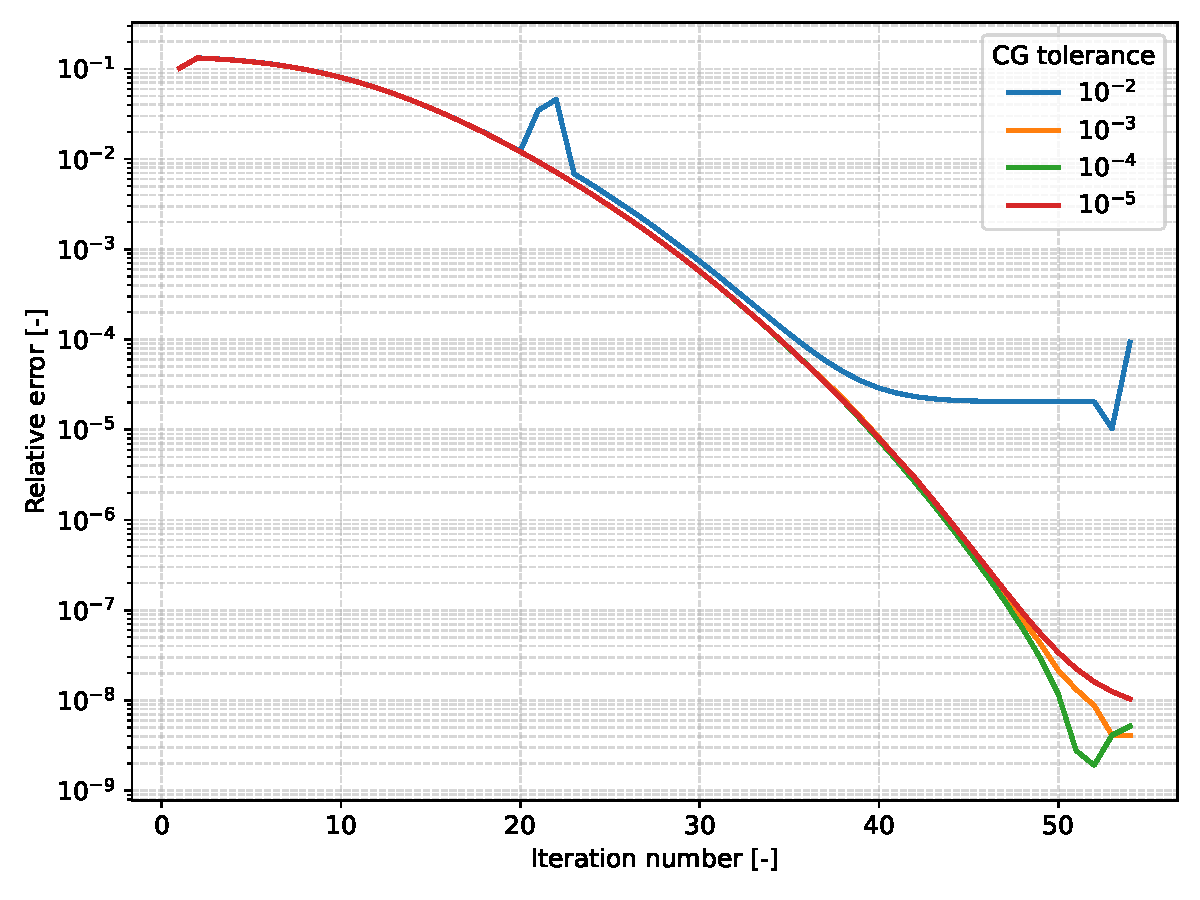
\includegraphics[width=0.9\textwidth]{Images/conv_tol.pdf}
    \caption{HF calculation convergence with varying CG tolerance for $^{16}$O, box $[-9, 9]$ fm, step size $0.3$ fm.} 
    \label{fig:conv_tol}
\end{figure}
\subsubsection{Inner GCG iterations}
The number of inner GCG maximum iterations, here named `inverse power steps' to avoid confusion, is slightly more nuanced than the CG tolerance. The algorithm converges to the true eigenpairs as the power steps are performed, so one could think that a higher number of steps would bring to HF convergence faster, since the precision on the eigenvalues increases, but this is not the case.
\\In figures \ref{fig:conv_steps_o} and \ref{fig:conv_steps_mg}, the convergence of the HF calculation is plotted for different number of steps, respectively, for the spherical nucleus $^{16}$O and the deformed nucleus $^{24}$Mg. 
\begin{figure}[h]
    \centering
    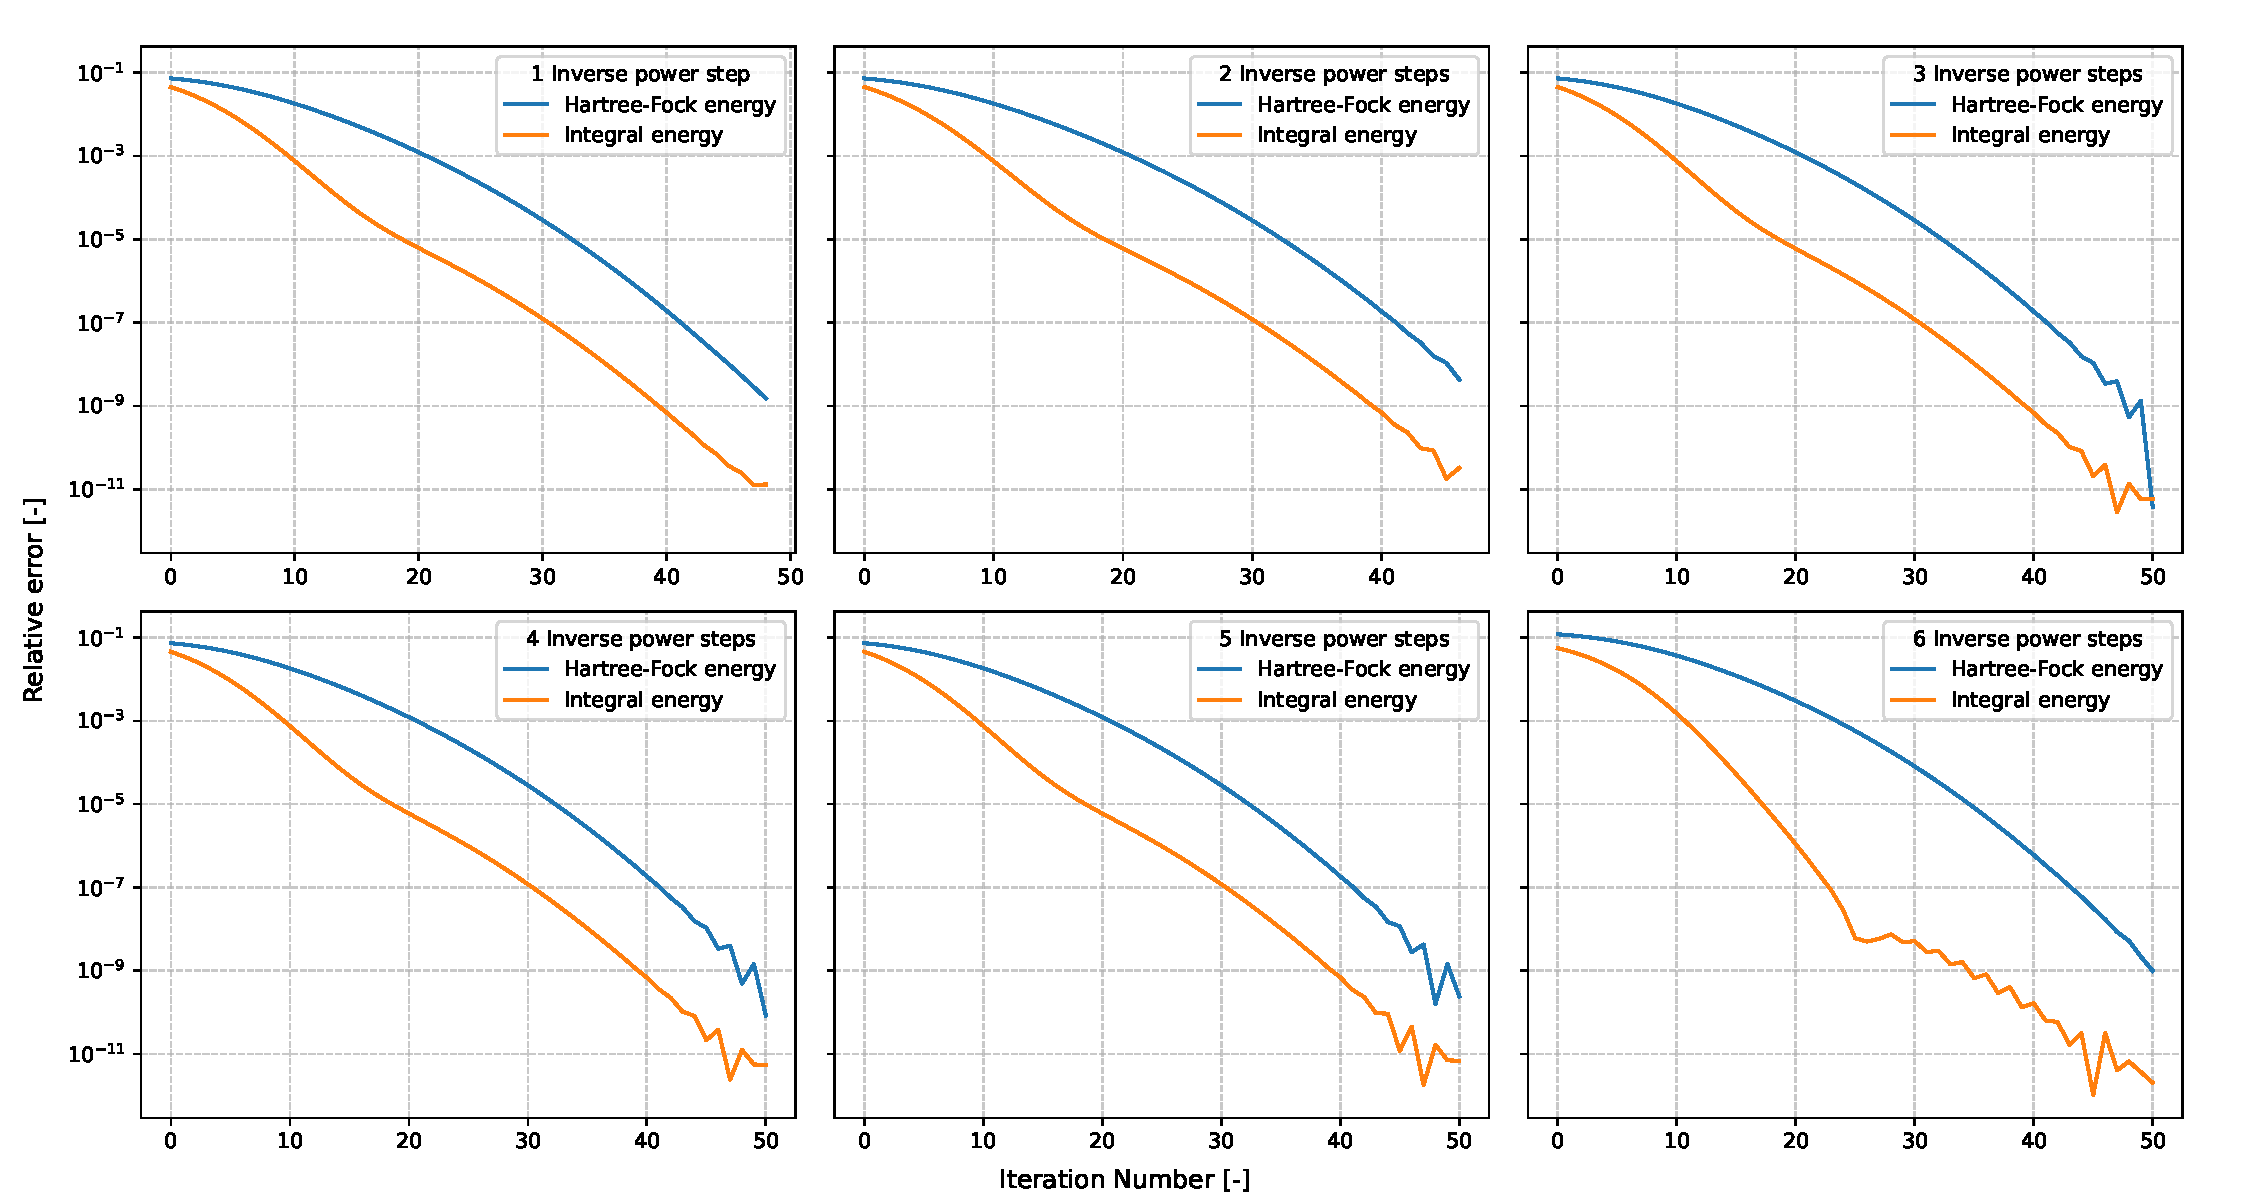
\includegraphics[width=1.0\textwidth]{Images/conv_steps_o.pdf}
    \caption{HF calculation convergence with varying number of inverse power steps for $^{16}$O, box $[-9, 9]$ fm, step size $0.3$ fm.}
    \label{fig:conv_steps_o}
\end{figure}
\begin{figure}[h]
    \centering
    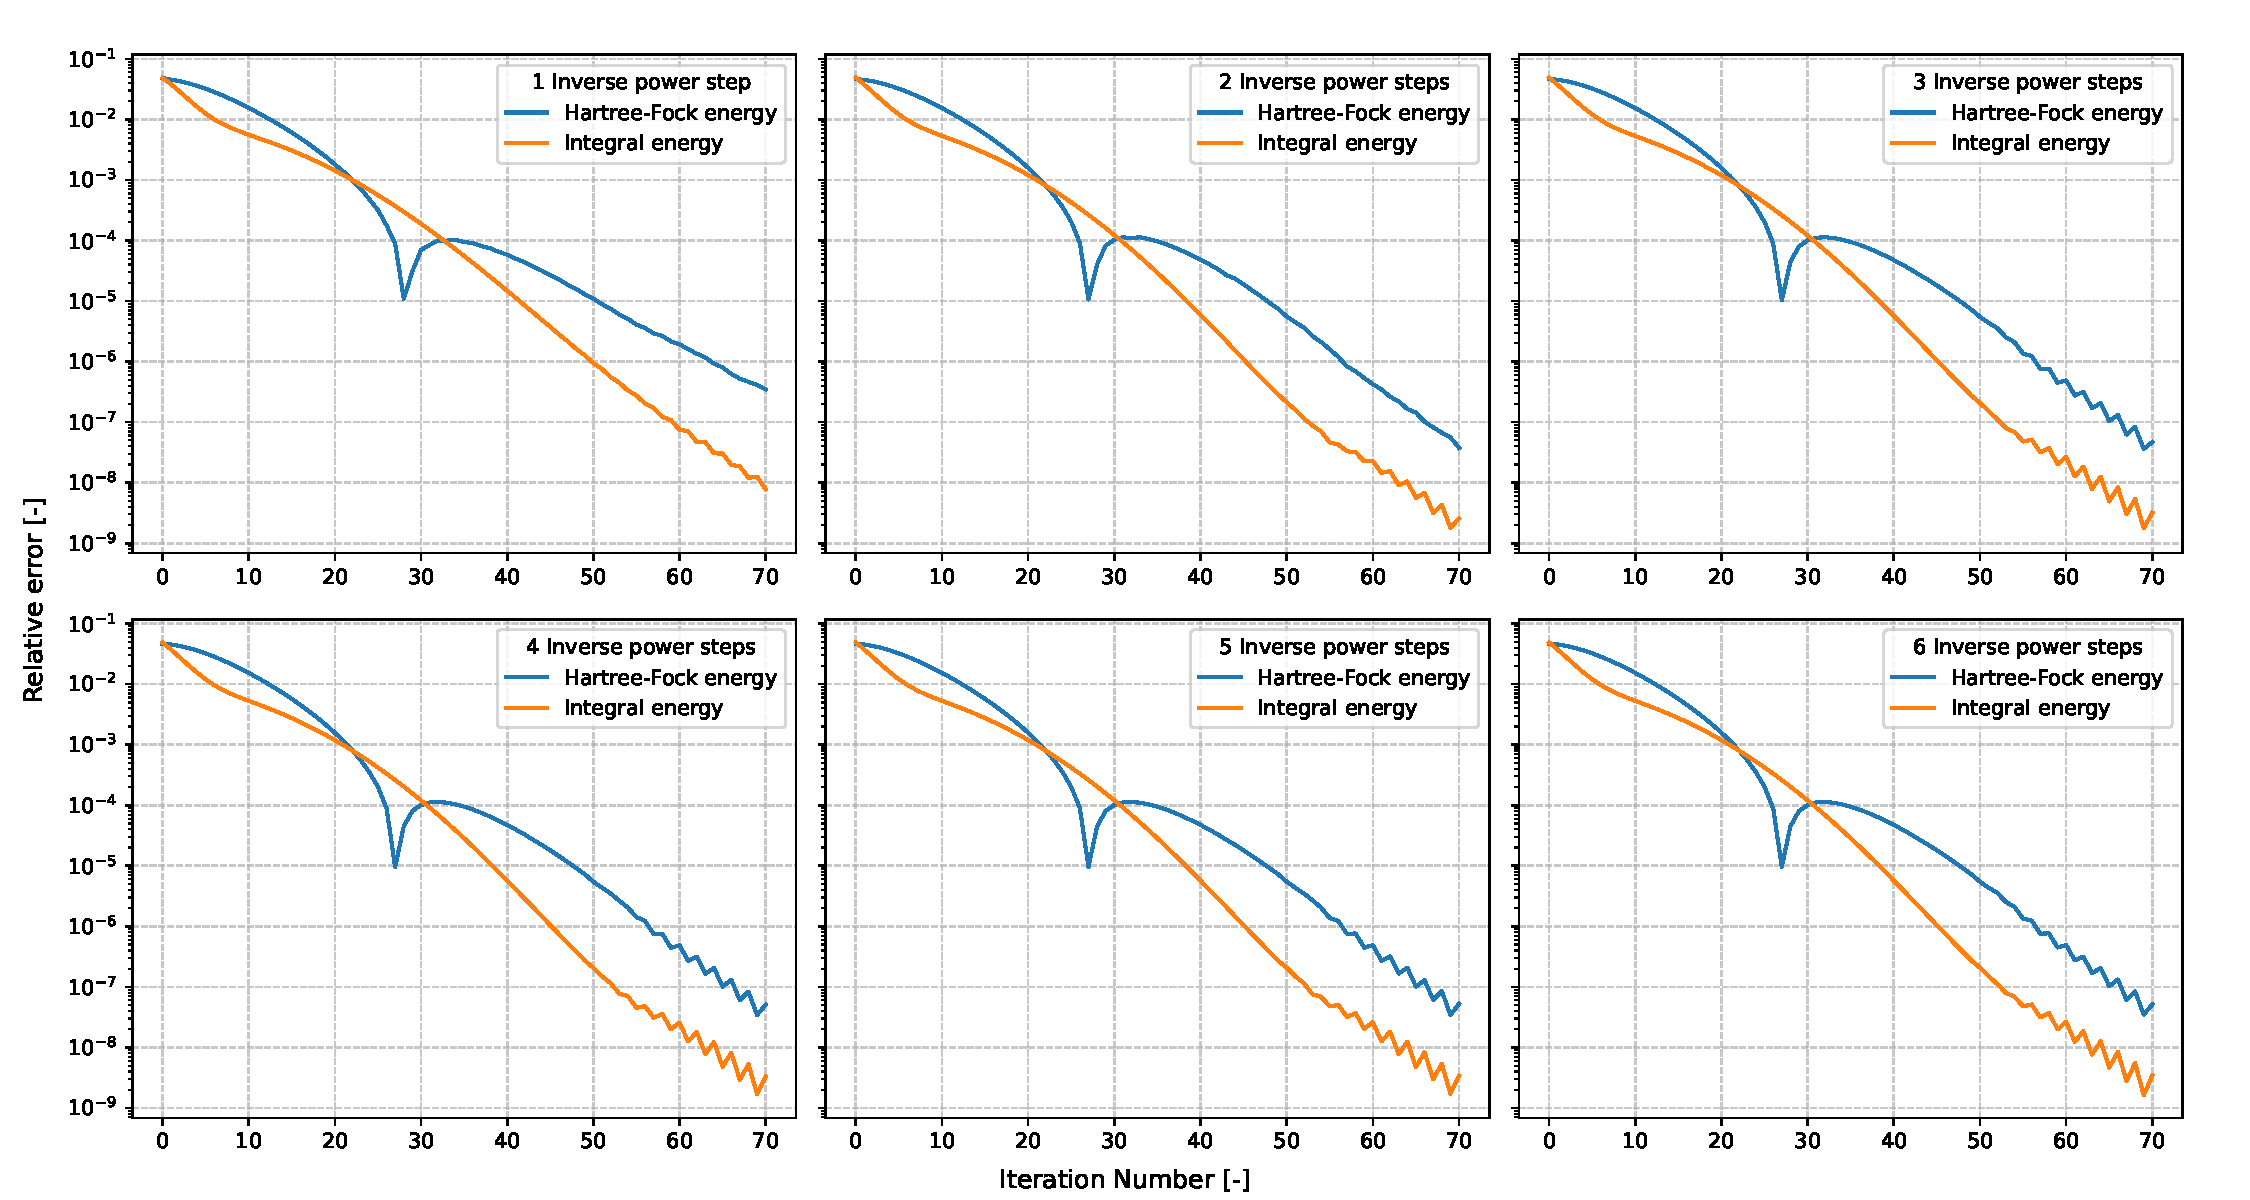
\includegraphics[width=1.0\textwidth]{Images/conv_steps.pdf}
    \caption{HF calculation convergence with varying number of inverse power steps for the deformed nucleus $^{24}$Mg, box $[-10, 10]$ fm, step size $0.33$ fm.}
    \label{fig:conv_steps_mg}
\end{figure}
It's evident that in both cases, a steps number greater than $3$ leads to oscillating behaviour near convergence, without accelerating it, while in the case of the spherical nucleus, just one step is enough to quickly, and reliably reach convergence. In any case, it's clear that delaying the inverse power steps to later HF iterations is safer in terms of stability.
\\This counter intuitive behavior is likely due to the fact that at each HF iteration the hamiltonian changes and a great number of steps leads to solutions too biased towards the current matrix eigenpairs, at the expense of the next iteration; however, in the case of deformed nuclei, due to sharp shape changes at the start of the calculation, just one step may not be enough to sustain the pace at which the Hamiltonian changes, hence the quicker convergence with more steps.




\subsection{Numerical stability}
As a final remark, the numerical stability of the solver is reported in figure \ref{fig:stability}. The map is produced for a spherical calculation of $^{16}$O, with varying box and mesh sizes. 
\\It's possible to observe that for a box whose side is at least $\approx 2.5$ times the nuclear radius, the solver numerical stability is loosely dependent on the box extension, but rather on the step size. This is not surprising, as the points separation in space $h$ dictates the precision of the discretized derivatives, as mentioned in section \ref{sec:finite_diff}.
\begin{figure}[H]
    \centering
    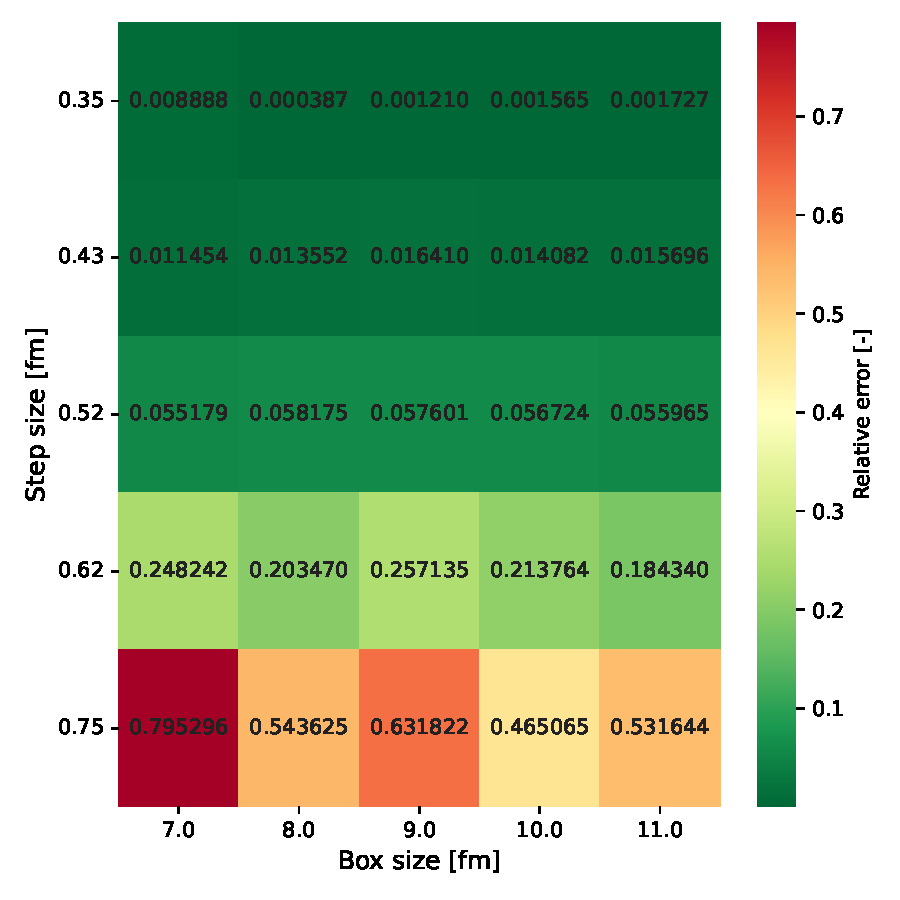
\includegraphics[width=1.0\textwidth]{Images/stability.pdf}
    \caption{Numerical stability map of the HF solver for $^{16}$O for different box and step sizes. Relative error is taken against a benchmark reference value.}
    \label{fig:stability}
\end{figure}
\section{Constraints}
\chapter{Results for spherical nuclei}
In this chapter, results for spherical nuclei are presented. These are mostly calculated for double magic nuclei, with the exception of $^{90}$Zr.
The reason behind choosing spherical nuclei as an initial benchmark, is that numerous spherical HF codes are available and they have the advantage of being one-dimensional, which allows the use of very fine meshes, with a step size that can go down to the physical scale of the problem, which is roughly 0.1 fm in this case, without any major computational limit. We can use these codes as a reference ideal value for the different quantities produced by our code. The choice for benchmarking spherical results in the present work has been the \texttt{hfbcs\_qrpa} code \cite{hfbcsqrpa}.
\section{Physical quantities}
After finding a nuclide's ground state, we are able to compute different physical properties of the system. We can use these values as a numerical reference when comparing our results with other codes.
\subsection{Mean square radii}
An important set of quantities characterizing the nuclear density is certainly the one of mean square radii.
The individual nuclear spieces' mean square radius is defined as
\begin{equation}
    \label{eq:msr}
    \expval{r^2_q} = \frac{\int\rho_q(\bm r) r^2 d\bm r}{\int \rho_q(\bm r) d\bm r}.
\end{equation}
While the charge mean square radius formula is derived from the convolution of the neutron and proton particle densities with their respective internal charge distribution \cite{BERTOZZI1972408}, resulting in equation \eqref{eq:cmsr}.
\begin{equation}
    \label{eq:cmsr}
    \expval{r^2_{ch}} = \expval{r^2_p} + \expval{r^2}_P + \frac N Z \expval{r^2}_N + \frac 2 Z \bigg(\frac{ \hbar}{mc}\bigg)^2\sum_{\alpha q}\mu_q \expval{\bm \sigma\cdot \bm {\ell}}_{\alpha q}
\end{equation}
where $q$ runs over the nuclear species and $\alpha$ runs over all single particle states of spcies $q$. $\bm \sigma$ is the vector operator of Pauli matrices, while $\bm {\ell}$ is the angular momentum operator $-i(\bm r \times \nabla)$.
$\expval{r^2}_P$ and $\expval{r^2}_N$ refer to the square charge radii of the proton and the neutron, while $\mu_q$ to their respective magnetic dipole moment in units of nuclear magneton.
\\All square charge radii computed in this work use the set of parameters in table \ref{tab:charge_par}, taken to be equal to the spherical benchmark code \texttt{hfbcs\_qrpa}.
\begin{table}[ht]
  \centering
  \begin{tabular}{lcc}
    \toprule
    \textbf{Parameter} & \textbf{Value} & \textbf{Units} \\
    \midrule
    $\expval{r^2}_P$ & 0.64 & fm$^2$ \\
    $\expval{r^2}_N$ & -0.11 & fm$^2$ \\
    $\mu_p$ & 2.792847 & - \\
    $\mu_n$ & -1.913043 & - \\
    \bottomrule
  \end{tabular}
  \caption{Parameters used to compute the charge mean square radius.}
  \label{tab:charge_par}
\end{table}
\subsection{Deformation parameters}
When dealing with deformed nuclei, mean square radii are not sufficient to characterize the nuclear density. The main parameter used is the quadrupole deformation parameter $\beta_2$, defined already in section (REF), it can be computed through the actual mean square radius with formula \eqref{eq:beta_real_radius}
\begin{equation}
    \label{eq:beta_real_radius}
    \beta_2 = \frac{4\pi\expval{Y_{2 0}}}{3A\expval{r^2}}
\end{equation}
where $\expval{r^2}$ is the total mean square radius of the nucleus 
\begin{equation}
    \expval{r^2} = \frac{\int (\rho_n + \rho_p )r^2 d\bm r}{\int (\rho_n + \rho_p )d\bm r} = \expval{x^2+y^2+z^2}.
\end{equation}
For spherical nuclei, $\beta_2 = 0$, while for deformed ones, thanks to the normalization with respect to the total radius and mass, the $\beta_2$ parameter can be used to compare different nuclei across the nuclide chart.
\section{Parameters and mesh choice}
All $\texttt{hfbcs\_qrpa}$ calculations were performed using a mesh size of $0.1$ fm, no pairing interaction, and a radial mesh size whose radius is equal to the side of the box in our computation. The lattice of our code depends on the extension of the nucleus, which is directly determined by its mass $A$; since the number of subdivisions that allows reasonable CPU times on a laptop caps around $60-70$, step sizes vary across different calculations. 
\\In the results shown here, for $^{16}$O, we are able to reach a $0.3$ fm step size, while for the heaviest, $^{90}$Zr, we are only able to reach $0.42$ fm. The reason behind this choice is that as the nucleus size increases, a bigger box is needed to ensure that all relevant states are able to decay to zero at the boundary. All the data reported in this chapter is computed with the SLy5 parametrization \cite{chabanat2}.
\section{Results for \(^{16}\)O}
The first results we will take a look at are the ones for $^{16}$O. It's the best candidate for gauging the solver's performance, as it is a very light, double magic nucleus, meaning it has no pairing interaction and a spherical shape.
\\All calculations are performed on a box of size $[-9, 9]$ fm in all three directions and a step size of $0.3$ fm, correponding to $2\cdot 60^{3}$ mesh points.
\subsection{Results neglecting Coulomb interaction}
Since the Skyrme functional is complex and nuanced, results are shown for more and more terms in expression \eqref{eq:skfunc}. We start by including only $C_0^\rho$, $C_1^\rho$, $C_0^\tau$, $C_1^\tau$ and neglecting the others and the Coulomb interaction; results are reported in table \ref{tab:no_so_no_j_no_coul}.
Without further terms, the spin-orbit field $\bm B(\bm r)$ vanishes, hence the $1p_{3/2}$ and $1p_{1/2}$ levels show degeneration in energy.
\\Since $N=Z$, assuming equal masses the single-particle equations will be exactly equal between the two species, therefore only neutron results are reported. Note that $C_1$ terms reduce to being null in this case, that is until we either break the $N=Z$ equality or introduce the Coulomb interaction.
\begin{table}[ht]
  \centering
  \begin{tabular}{lrrccc}
    \multicolumn{6}{c}{\textbf{Physical quantities}}\\
    \addlinespace[0.3em]
    \toprule
    && GCG & hfbcs\_qrpa & $\Delta$ & $\Delta\%$ \\
    \midrule
    $E_{\text{TOT}}$& [MeV] & -141.582 & -141.582 & - & - \\
    $\expval{ r^2_n}^{1/2}$ &[fm] & 2.6504 & 2.6510 & 0.0006 & \num{2.26e-2}\\
    $\expval{ r^2_{ch}}^{1/2}$ &[fm] & 2.7486 & 2.7491 & 0.0005 & \num{1.82e-2}\\
    \midrule
    \addlinespace[1.3em]
    \multicolumn{6}{c}{\textbf{Neutron energy levels}}\\
    \addlinespace[0.3em]
    \midrule
    && GCG & hfbcs\_qrpa & $\Delta$ & $\Delta\%$ \\
    \midrule
    1s$_{1/2}$ &[MeV] & -36.142 & -36.139 & 0.003 & \num{8.30e-3}\\
    1p$_{3/2}$ &[MeV] & -18.573 & -18.572 & 0.001 & \num{5.38e-3}\\
    1p$_{1/2}$ &[MeV] & -18.573 & -18.572 & 0.001 & \num{5.38e-3}\\
    \bottomrule
  \end{tabular}
  \caption{$^{16}$O including $C_0^{\rho}$, $C_1^{\rho}$, $C_0^{\tau}$, $C_1^{\tau}$ terms, neglecting Coulomb interaction.}
  \label{tab:no_so_no_j_no_coul}
\end{table}
In table \ref{tab:compare_so} the $C_0^{\div \bm J}$ and $C_1^{\div \bm J}$ terms are included just for the spin-orbit field $\bm B(\bm r)$, but not for the mean field $U(\bm r)$; from an interaction point of view, it's as if we were neglecting the spin-gradient coupling term \cite{chabanat2}. As expected, the $1p_{3/2}$ and $1p_{1/2}$ degeneration is removed, displaying the spin-orbit splitting, which lowers the total angular momentum $j=3/2$ level and raises the $j=1/2$ level.
\begin{table}[ht]
  \centering
  \begin{tabular}{lrrccc}
    \multicolumn{6}{c}{\textbf{Physical quantities}}\\
    \addlinespace[0.3em]
    \toprule
    && GCG & hfbcs\_qrpa & $\Delta$ & $\Delta\%$ \\
    \midrule
    $E_{\text{TOT}}$& [MeV] & -142.080 & -142.080 & - & - \\
    $\expval{ r^2_n}^{1/2}$ &[fm] & 2.6516 & 2.6516 & - & -\\
    $\expval{ r^2_{ch}}^{1/2}$ &[fm] & 2.7497 & 2.7497 & - & -\\
    \midrule
    \addlinespace[1.3em]
    \multicolumn{6}{c}{\textbf{Neutron energy levels}}\\
    \addlinespace[0.3em]
    \midrule
    && GCG & hfbcs\_qrpa & $\Delta$ & $\Delta\%$ \\
    \midrule
    1s$_{1/2}$ &[MeV] & -36.314 & -36.312 & 0.002 & \num{5.5e-3}\\
    1p$_{3/2}$ &[MeV] & -20.696 & -20.696 & - & -\\
    1p$_{1/2}$ &[MeV] & -14.335 & -14.335 & - & -\\
    \bottomrule
  \end{tabular}
  \caption{$^{16}$O including $C_0^\rho$, $C_1^\rho$, $C_0^\tau$, $C_1^\tau$, $C_0^{\div \bm J}$, $C_1^{\div \bm J}$ terms, neglecting Coulomb interaction and $J^2$ terms.}
  \label{tab:compare_so}
\end{table}
\\Lastly, the $C_0^{\div \bm J}$ and $C_1^{\div \bm J}$ terms are also included in the calculation of the mean-field, resulting in the full implementation of the Skyrme functional. As shown in table \ref{tab:compare_j2}, the effect of this addition on the ground state is little, as the spin current $J_{\mu \nu}$ is small in light, closed shell nuclei.
\begin{table}[ht]
  \centering
  \begin{tabular}{lrrccc}
    \multicolumn{6}{c}{\textbf{Physical quantities}}\\
    \addlinespace[0.3em]
    \toprule
    && GCG & hfbcs\_qrpa & $\Delta$ & $\Delta\%$ \\
    \midrule
    $E_{\text{TOT}}$& [MeV] & -142.074 & -142.074 & - & - \\
    $\expval{ r^2_n}^{1/2}$ &[fm] & 2.6515 & 2.6516 & 0.0001 & \num{3.77e-3}\\
    $\expval{ r^2_{ch}}^{1/2}$ &[fm] & 2.7497 & 2.7497 & - & -\\
    \midrule
    \addlinespace[1.3em]
    \multicolumn{6}{c}{\textbf{Neutron energy levels}}\\
    \addlinespace[0.3em]
    \midrule
    && GCG & hfbcs\_qrpa & $\Delta$ & $\Delta\%$ \\
    \midrule
    1s$_{1/2}$ &[MeV] & -36.309 & -36.308 & 0.001 & \num{2.75e-3}\\
    1p$_{3/2}$ &[MeV] & -20.684 & -20.685 & 0.001 & \num{4.83e-3}\\
    1p$_{1/2}$ &[MeV] & -14.361 & -14.361 & - & -\\
    \bottomrule
  \end{tabular}
  \caption{$^{16}$O neglecting Coulomb interaction.}
  \label{tab:compare_j2}
\end{table}
\subsubsection{Results including Coulomb interaction}
As the final addition to get a complete and accurate description of $^{16}$O, the Coulomb interaction is included as detailed in section \ref{sec:coulomb_treatment}. Results are shown in table \ref{tab:confronto}.
\begin{table}[ht]
  \centering
  \begin{tabular}{lrrccc}
    \multicolumn{6}{c}{\textbf{Physical quantities}}\\
    \addlinespace[0.3em]
    \toprule
    && GCG & hfbcs\_qrpa & $\Delta$ & $\Delta\%$ \\
    \midrule
    $E_{\text{TOT}}$& [MeV] & -128.402 & -128.400 & 0.002 & \num{1.56e-3} \\
    $\expval{ r^2_n}^{1/2}$ &[fm] & 2.6584 & 2.6585 & 0.0001 & \num{3.76e-3}\\
    $\expval{ r^2_p}^{1/2}$ &[fm] & 2.6835 & 2.6836 & 0.0001 & \num{3.73e-3}\\
    $\expval{ r^2_{ch}}^{1/2}$ &[fm] & 2.7805 & 2.7803 & 0.0002 & \num{7.19e-3}\\
    \midrule
    \addlinespace[1.3em]
    \multicolumn{6}{c}{\textbf{Neutron energy levels}}\\
    \addlinespace[0.3em]
    \midrule
    && GCG & hfbcs\_qrpa & $\Delta$ & $\Delta\%$ \\
    \midrule
    1s$_{1/2}$ &[MeV] & -36.140 & -36.137 & 0.003 & \num{8.30e-3}\\
    1p$_{3/2}$ &[MeV] & -20.611 & -20.611 & - & -\\
    1p$_{1/2}$ &[MeV] & -14.427 & -14.428 & 0.001 & \num{6.93e-3}\\
    \midrule
    \addlinespace[1.3em]
    \multicolumn{6}{c}{\textbf{Proton energy levels}}\\
    \addlinespace[0.3em]
    \midrule
    && GCG & hfbcs\_qrpa & $\Delta$ & $\Delta\%$ \\
    \midrule
    1s$_{1/2}$ &[MeV] & -32.349 & -32.345 & 0.004 & \num{1.24e-2}\\
    1p$_{3/2}$ &[MeV] & -17.137 & -17.137 & - & -\\
    1p$_{1/2}$ &[MeV] & -11.081 & -11.082 & 0.001 & \num{9.02e-3}\\
    \bottomrule
  \end{tabular}
  \caption{$^{16}$O complete of the Skyrme functional and Coulomb interaction.}
  \label{tab:confronto}
\end{table}
\\As shown in tables \ref{tab:no_so_no_j_no_coul}, \ref{tab:compare_so}, \ref{tab:compare_j2}, and \ref{tab:confronto} results for $^{16}$O are in great agreement with the output of the \texttt{hfbcs\_qrpa} code for all the terms in the Skyrme functional.
\section{Results for heavier nuclei}
In the following section, results for some spherical nuclei heavier than $^{16}$O are presented in tables \ref{tab:compare_all_ca48}, \ref{tab:compare_all_ni56} and \ref{tab:compare_all_zr90}.
Our code still shows good agreement with the \texttt{hfbcs\_qrpa} one. A slight increase of the numerical error can be observed as the step size increaseas, which is compatible with the polynomial error in the finite difference method.
\begin{table}[ht]
  \centering
  \begin{tabular}{lrrccc}
    \multicolumn{6}{c}{\textbf{Physical quantities}}\\
    \addlinespace[0.3em]
    \toprule
    && GCG & hfbcs\_qrpa & $\Delta$ & $\Delta\%$ \\
    \midrule
    $E_{\text{TOT}}$& [MeV] & -415.955 & -415.931 & 0.024 & \num{5.77e-3} \\
    $\expval{ r^2_n}^{1/2}$ &[fm] & 3.6106 & 3.6110 & 0.0004 & \num{1.11e-2}\\
    $\expval{ r^2_p}^{1/2}$ &[fm] & 3.4502 & 3.4507 & 0.0005 & \num{1.45e-2}\\
    $\expval{ r^2_{ch}}^{1/2}$ &[fm] & 3.5274 & 3.5060 & 0.0214 & 0.610\\
    \midrule
    \addlinespace[1.3em]
    \multicolumn{6}{c}{\textbf{Neutron energy levels}}\\
    \addlinespace[0.3em]
    \midrule
    && GCG & hfbcs\_qrpa & $\Delta$ & $\Delta\%$ \\
    \midrule
    1s$_{1/2}$ &[MeV] & -49.758 & -49.752 & 0.006 & \num{1.21e-2}\\
    1p$_{3/2}$ &[MeV] & -35.952 & -35.949 & 0.003 & \num{8.34e-3}\\
    1p$_{1/2}$ &[MeV] & -33.891 & -33.891 & - & -\\
    1d$_{5/2}$ &[MeV] & -22.170 & -22.169 & 0.001 & \num{4.51e-3}\\
    2s$_{1/2}$ &[MeV] & -17.720 & -17.720 & - & -\\
    1d$_{3/2}$ &[MeV] & -17.431 & -17.434 & 0.003 & \num{1.72e-2}\\
    1f$_{7/2}$ &[MeV] & -9.262 & -9.261 & 0.001 & \num{1.08e-2}\\
    \midrule
    \addlinespace[1.3em]
    \multicolumn{6}{c}{\textbf{Proton energy levels}}\\
    \addlinespace[0.3em]
    \midrule
    && GCG & hfbcs\_qrpa & $\Delta$ & $\Delta\%$ \\
    \midrule
    1s$_{1/2}$ &[MeV] & -45.936 & -45.930 & 0.006 & \num{1.31e-2}\\
    1p$_{3/2}$ &[MeV] & -34.314 & -34.311 & 0.003 & \num{8.74e-3}\\
    1p$_{1/2}$ &[MeV] & -30.482 & -30.483 & 0.001 & \num{3.28e-3}\\
    1d$_{5/2}$ &[MeV] & -22.455 & -22.454 & 0.001 & \num{4.45e-3}\\
    2s$_{1/2}$ &[MeV] & -16.753 & -16.751 & 0.002 & \num{1.19e-2}\\
    1d$_{3/2}$ &[MeV] & -15.337 & -15.340 & 0.003 & \num{1.96e-2}\\
    \bottomrule
  \end{tabular}
  \caption{$^{48}$Ca, box size [-12, 12] fm, step size 0.34 fm}
  \label{tab:compare_all_ca48}
\end{table}

\begin{table}[ht]
  \centering
  \begin{tabular}{lrrccc}
    \multicolumn{6}{c}{\textbf{Physical quantities}}\\
    \addlinespace[0.3em]
    \toprule
    && GCG & hfbcs\_qrpa & $\Delta$ & $\Delta\%$ \\
    \midrule
    $E_{\text{TOT}}$& [MeV] & -482.805 & -482.700 & 0.105 & \num{2.18e-2} \\
    $\expval{ r^2_n}^{1/2}$ &[fm] & 3.6422 & 3.6433 & 0.0011 & \num{3.02e-2}\\
    $\expval{ r^2_p}^{1/2}$ &[fm] & 3.6968 & 3.6979 & 0.0011 & \num{2.97e-2}\\
    $\expval{ r^2_{ch}}^{1/2}$ &[fm] & 3.7722 & 3.7682 & 0.0040 & 0.106\\
    \midrule
    \addlinespace[1.3em]
    \multicolumn{6}{c}{\textbf{Neutron energy levels}}\\
    \addlinespace[0.3em]
    \midrule
    && GCG & hfbcs\_qrpa & $\Delta$ & $\Delta\%$ \\
    \midrule
    1s$_{1/2}$ &[MeV] & -54.277 & -54.260 & 0.017 & \num{3.13e-2}\\
    1p$_{3/2}$ &[MeV] & -41.571 & -41.562 & 0.009 & \num{2.16e-2}\\
    1p$_{1/2}$ &[MeV] & -39.613 & -39.611 & 0.002 & \num{5.05e-3}\\
    1d$_{5/2}$ &[MeV] & -28.536 & -28.530 & 0.006 & \num{2.10e-2}\\
    2s$_{1/2}$ &[MeV] & -23.539 & -23.545 & 0.006 & \num{2.55e-2}\\
    1d$_{3/2}$ &[MeV] & -23.367 & -23.361 & 0.006 & \num{2.57e-2}\\
    1f$_{7/2}$ &[MeV] & -16.019 & -16.018 & 0.001 & \num{6.24e-3}\\
    \midrule
    \addlinespace[1.3em]
    \multicolumn{6}{c}{\textbf{Proton energy levels}}\\
    \addlinespace[0.3em]
    \midrule
    && GCG & hfbcs\_qrpa & $\Delta$ & $\Delta\%$ \\
    \midrule
    1s$_{1/2}$ &[MeV] & -43.754 & -43.740 & 0.014 & \num{3.20e-2}\\
    1p$_{3/2}$ &[MeV] & -31.561 & -31.555 & 0.006 & \num{1.90e-2}\\
    1p$_{1/2}$ &[MeV] & -29.545 & -29.545 & - & -\\
    1d$_{5/2}$ &[MeV] & -19.017 & -19.016 & 0.001 & \num{5.26e-3}\\
    2s$_{1/2}$ &[MeV] & -14.004 & -14.012 & 0.008 & \num{5.71e-2}\\
    1d$_{3/2}$ &[MeV] & -13.891 & -13.887 & 0.004 & \num{2.88e-2}\\
    1f$_{7/2}$ &[MeV] & -6.934 & -6.935 & 0.001 & \num{1.44e-2}\\
    \bottomrule
  \end{tabular}
  \caption{$^{56}$Ni, box size [-13, 13] fm, step size 0.37 fm}
  \label{tab:compare_all_ni56}
\end{table}

\begin{table}[ht]
  \centering
  \begin{tabular}{lrrccc}
    \multicolumn{6}{c}{\textbf{Physical quantities}}\\
    \addlinespace[0.3em]
    \toprule
    && GCG & hfbcs\_qrpa & $\Delta$ & $\Delta\%$ \\
    \midrule
    $E_{\text{TOT}}$& [MeV] & -783.587 & -783.325 & 0.262 & \num{3.34e-2} \\
    $\expval{ r^2_n}^{1/2}$ &[fm] & 4.2854 & 4.2872 & 0.0018 & \num{4.20e-2}\\
    $\expval{ r^2_p}^{1/2}$ &[fm] & 4.2196 & 4.2212 & 0.0016 & \num{3.79e-2}\\
    $\expval{ r^2_{ch}}^{1/2}$ &[fm] & 4.2767 & 4.2704 & 0.0063 & 0.148\\
    \midrule
    \addlinespace[1.3em]
    \multicolumn{6}{c}{\textbf{Neutron energy levels}}\\
    \addlinespace[0.3em]
    \midrule
    && GCG & hfbcs\_qrpa & $\Delta$ & $\Delta\%$ \\
    \midrule
    1s$_{1/2}$ &[MeV] & -55.636 & -55.615 & 0.021 & \num{3.78e-2}\\
    1p$_{3/2}$ &[MeV] & -45.324 & -45.309 & 0.015 & \num{3.31e-2}\\
    1p$_{1/2}$ &[MeV] & -44.172 & -44.160 & 0.012 & \num{2.72e-2}\\
    1d$_{5/2}$ &[MeV] & -34.148 & -34.137 & 0.011 & \num{3.22e-2}\\
    2s$_{1/2}$ &[MeV] & -31.393 & -31.391 & 0.002 & \num{6.37e-3}\\
    1d$_{3/2}$ &[MeV] & -29.802 & -29.797 & 0.005 & \num{1.68e-2}\\
    1f$_{7/2}$ &[MeV] & -22.755 & -22.748 & 0.007 & \num{3.08e-2}\\
    2p$_{3/2}$ &[MeV] & -17.837 & -17.840 & 0.003 & \num{1.68e-2}\\
    1f$_{5/2}$ &[MeV] & -17.568 & -17.563 & 0.005 & \num{2.85e-2}\\
    2p$_{1/2}$ &[MeV] & -15.729 & -15.723 & 0.006 & \num{3.82e-2}\\
    1g$_{9/2}$ &[MeV] & -11.586 & -11.580 & 0.006 & \num{5.18e-2}\\
    \midrule
    \addlinespace[1.3em]
    \multicolumn{6}{c}{\textbf{Proton energy levels}}\\
    \addlinespace[0.3em]
    \midrule
    && GCG & hfbcs\_qrpa & $\Delta$ & $\Delta\%$ \\
    \midrule
    1s$_{1/2}$ &[MeV] & -44.973 & -44.956 & 0.017 & \num{3.78e-2}\\
    1p$_{3/2}$ &[MeV] & -36.347 & -36.336 & 0.011 & \num{3.03e-2}\\
    1p$_{1/2}$ &[MeV] & -34.121 & -34.115 & 0.006 & \num{1.76e-2}\\
    1d$_{5/2}$ &[MeV] & -26.766 & -26.759 & 0.007 & \num{2.62e-2}\\
    2s$_{1/2}$ &[MeV] & -22.175 & -22.178 & 0.003 & \num{1.35e-2}\\
    1d$_{3/2}$ &[MeV] & -21.216 & -21.214 & 0.002 & \num{9.43e-3}\\
    1f$_{7/2}$ &[MeV] & -16.722 & -16.718 & 0.004 & \num{2.39e-2}\\
    2p$_{3/2}$ &[MeV] & -10.239 & -10.236 & 0.003 & \num{2.93e-2}\\
    1f$_{5/2}$ &[MeV] & -9.613 &  -9.618 & 0.005 & \num{5.20e-2}\\
    2p$_{1/2}$ &[MeV] & -8.108 &  -8.104 & 0.004 & \num{4.94e-2}\\
    \bottomrule
  \end{tabular}
  \caption{$^{90}$Zr, box size [-15, 15] fm, step size 0.43 fm}
  \label{tab:compare_all_zr90}
\end{table}
\subsection{Comparison with experimental binding energies}
The Skyrme functional is highly successful at producing theoretical values in great accordance with experimental data, just by fitting a small set of parameters \cite{Bender2003}. In table \ref{tab:exp_comp}, binding energies of some of the nuclei studied in this work are compared with experimental values, taken from the Atomic Mass Data Center \cite{AMDC_website}.
\begin{table}[ht]
  \centering
  \begin{tabular}{lcccc}
    \toprule
    &$^{16}$O&$^{48}$Ca&$^{56}$Ni&$^{90}$Zr\\
    \midrule
    $E_{\text{th}}$ & 128.40 & 415.95 & 482.80 & 783.59 \\
    $E_{\text{exp}}$ & 127.62 & 414.33 & 483.99 & 783.89 \\ 
    \bottomrule
    \end{tabular}
    \caption{Comparison of experimental binding energies in MeV with theoretical calculated values using the SLy5 functional.}
    \label{tab:exp_comp}
  \end{table}
\chapter{Results for deformed nuclei}
Having established that the code works well for spherical nuclei, we can start treading in deformation territory.
\section{$^{24}$Mg}
In the following section, results for $^{24}$Mg are presented, it's a natural choice to study how well deformations are represented by our framework, since it's light, very deformed and shows no pairing interaction in its ground state.
\subsection{\texttt{HFBTHO} code and calculation details}
\subsubsection{\texttt{HFBTHO}}
To benchmark the code in the case of nuclear deformation, the \texttt{HFBTHO} code was used \cite{MAREVIC2022108367}, it's a HFB code which minimizes the energy functional on a (Transformed) harmonic oscillator basis. Since $^{24}$Mg is a light nucleus, it still works well in this case.
All calculations were performed using 12 oscillator shells and assuming a zero pairing interaction. 
Default parameters were adopted for the quadrupole constraints. 
Since the version of \texttt{HFBTHO} used in this work has been compiled with the $J^2$ terms disabled, we present the results from our code both with and without them. 
The results obtained without them serve as a benchmark for the code, 
while those including the $J^2$ contribution illustrate their impact on the calculated observables.
\subsubsection{Code parameters and axial constraint}
As for our code, calculations are performed on a box $[-10, 10]$ fm.
In the case of the ground state calculation, a step size of $0.33$ fm is used, with a starting guess of a deformed Woods-Saxon with $\beta_2=0.4$.
\\The calculation in the case of the deformation curve is carried out imposing the following constraints
\begin{align}
  \expval{\Re\mathcal Q_{22}} = 0
  \\\expval{\Im \mathcal Q_{22}} = 0
  \\\expval{Y_{20}} = q_{20}.
\end{align}
These constraints altogether impose an axial deformation on the system. This is done because on a full mesh like in our case, the nucleus may deform on a different axis from the chosen one (z), resulting in spurious contributions to the real deformation curve; moreover, the axial symmetry of $\texttt{HFBTHO}$ doesn't allow broken axial symmetry configurations.
\\Regarding the stiffness $c$ and damping parameter $\mu$ of ALM in section \ref{sec:alm}, $c=0.001$ and $\mu=0.1$ were used. As for convergence criteria, a tolerance of $0.001$ on the value of $\beta_2 - \beta_{2, \text{target}}$ was used.
\subsubsection{Ground state}
Table \ref{tab:mg_table} reports data of the comparison for the ground state of $^{24}$Mg, while figure \ref{fig:mg_gs_density_axial} shows the middle section of the total particle density.
Charge radii for the two codes are displayed but not compared, due to different formulas used for their computation. $\expval{x^2}, \expval{y^2}$ and $\expval{z^2}$ is reported for our code but not for \texttt{HFBTHO} since it doesn't compute them.
\begin{table}[ht]
  \centering
  \begin{tabular}{lrccccc}
    \addlinespace[0.3em]
    \toprule
    && GCG & GCG no $J^2$ & \texttt{HFBTHO} & $\Delta$ & $\Delta\%$ \\
    \midrule
    $E_{\text{TOT}}$& [MeV]    & -195.854 & -197.219 &-197.030 & 0.189 & \num{9.52e-2} \\
    $\expval{ r^2_n}^{1/2}$    &[fm] & 3.0124 & 2.9998    & 2.9996 & 0.0002  & \num{6.67e-3}\\
    $\expval{ r^2_p}^{1/2}$    &[fm] & 3.0475 & 3.0346    & 3.0326  & 0.0020 & \num{6.59e-2}\\
    $\expval{ r^2_{ch}}^{1/2}$ &[fm] & 3.1364 & 3.1240    & 3.4614  & - & - \\
    $\expval{z^2}^{1/2}$ &[fm] & 2.145 &2.128 &- &-&-\\
    $\expval{x^2}^{1/2}$ &[fm] & 1.511 &1.511 & -&-&-\\
    $\expval{y^2}^{1/2}$ &[fm] & 1.514 &1.514 & -&-&-\\
    $\beta_2$ &[-] & 0.399 &0.390 & 0.390 & - & -  \\
    \bottomrule
  \end{tabular}
  \caption{Results for $^{24}$Mg ground state, no pairing interaction, box $[-10, 10]$ fm, step size 0.33 fm, SKM* parametrization.}
  \label{tab:mg_table}
\end{table}
\\The comparison shows good agreement between the two codes, with the same $\beta_2$ minimum and similar ground state properties.
\begin{figure}[h]
  \centering
  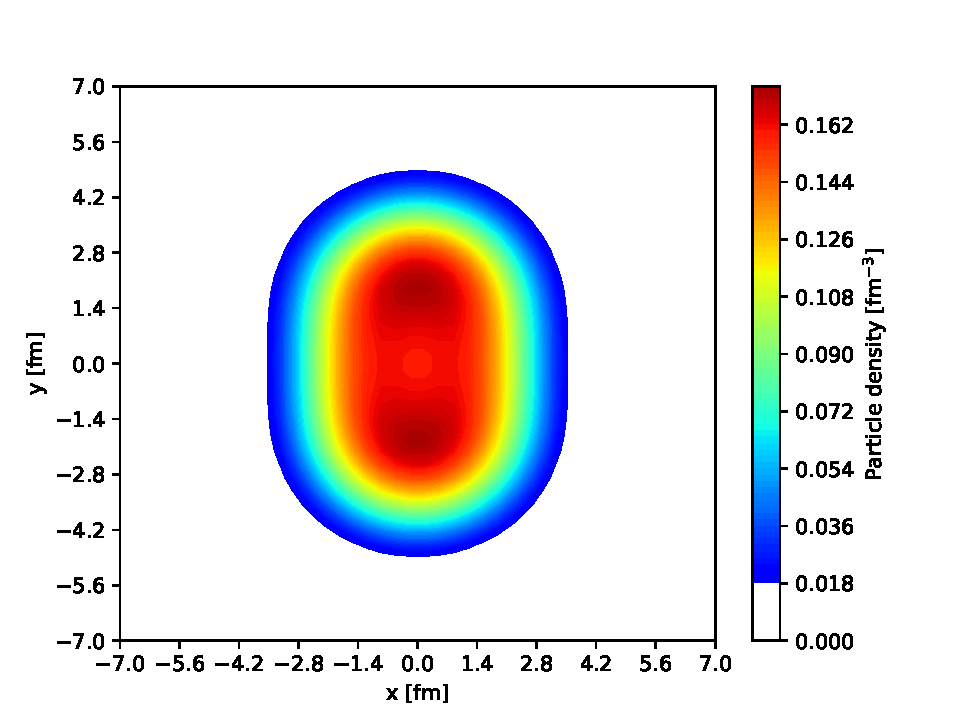
\includegraphics[width=1.0\linewidth]{Images/mg_gs_density_axial.pdf}
  \caption{Magnesium ground state density $\rho(x, y, 0)$, calculation done on a box $[-10, 10]$ fm, step size 0.33 fm, SKM* parametrization}
  \label{fig:mg_gs_density_axial}
\end{figure}
\subsubsection{Deformation curve}
In figure \ref{fig:mg_no_pair_deformation}, the deformation curve is shown for $^{24}$Mg, without pairing. To counteract the sharp rise in CPU time, due to the high number of points in the curve, a coarser lattice than the one in the ground state calculation is used, hence the shift in energy of the curve.
\begin{figure}[h]
  \centering
  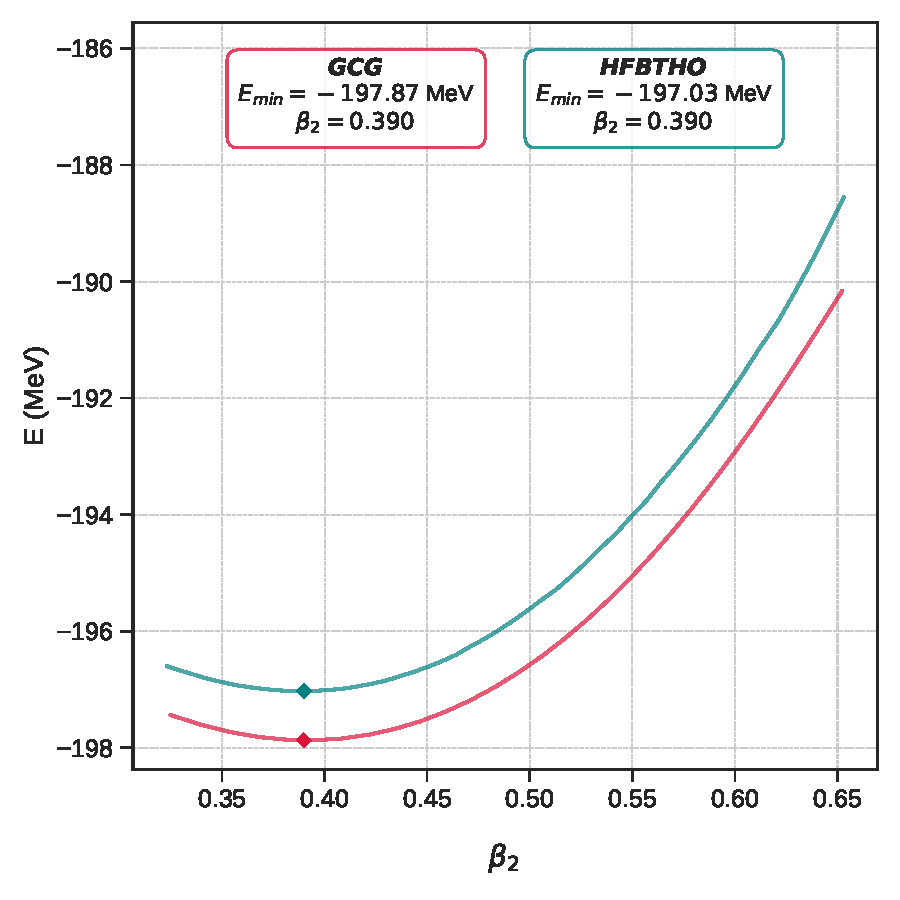
\includegraphics[width=0.8\linewidth]{Images/mg_nopair_curve.pdf}
  \caption{Magnesium deformation curve, no pairing interaction, calculation done on a box $[-10, 10]$ fm, step size 0.66 fm, SKM* parametrization, neglecting $J^2$ terms.}
  \label{fig:mg_no_pair_deformation}
\end{figure}
\\Figure \ref{fig:mg_no_pair_deformation} shows the same trend for both codes, with a minimum of the energy in $\beta_2=0.390$, albeit a difference in the energies due to the corase mesh, a gap which is shown in table \ref{tab:mg_table} to shrink when increasing the accuracy of the step size.

\addtocontents{toc}{\vspace{2em}} % Add a gap in the Contents, for aesthetics
\bibliography{Thesis_bibliography} % The references information are stored in the file named "Thesis_bibliography.bib"

%-------------------------------------------------------------------------
%	APPENDICES
%-------------------------------------------------------------------------

\cleardoublepage
\addtocontents{toc}{\vspace{2em}} % Add a gap in the Contents, for aesthetics
\appendix
\chapter{Appendix}
\section{Spherical harmonics}
\label{sec:spherical_harmonics}
Spherical harmonics, of order $\lambda, \mu$, are defined as
\begin{equation}
    Y_{\lambda\mu} (\theta, \phi) = (-1)^\mu 
    \sqrt{\frac{2\lambda + 1}{4\pi}\frac{(\lambda-\mu)!}{(\lambda+\mu)!}}
    \, P_\lambda^\mu(\cos\theta) \, e^{i\mu\phi}.
\end{equation}
Being able to provide the expression for arbitrary $\mu, \lambda$ through an algorithm 
is important in the current framework, to solve the Poisson equation and investigate 
nuclear properties.
\\The major challenge is to generate the associated Legendre polynomials $P_\lambda^\mu$.
They can be expressed in the form (for positive $\mu$)
\begin{equation}
    P_\lambda^\mu(x) = (1-x^2)^{\mu/2} \dv[\mu]{P_\lambda(x)}{x},
\end{equation}
where $x = \cos\theta$ and
\begin{equation}
    P_\lambda(x) = \frac 1 {2^\lambda \lambda !}
    \dv[\lambda]{(x^2-1)^\lambda}{x}.
\end{equation}
To compute the arbitrary $\lambda, \mu$ associated Legendre polynomial we can employ a recursive approach, setting $\lambda =\mu$
\begin{equation}
    P_\mu^\mu(x) = (2\mu-1)!! \, (1-x^2)^{\mu/2},
\end{equation}
where $(2\mu-1)!! = 1\cdot 3 \cdot 5 \ldots (2\mu-1)$ denotes the double factorial.
Once $P_\mu^\mu(x)$ is known, the next element with $\lambda = \mu +1$ reads
\begin{equation}
    P_{\mu+1}^\mu(x) = x(2\mu+1)P_\mu^\mu(x).
\end{equation}
All higher orders are then generated using the standard upward recurrence relation in $\lambda$:
\begin{equation}
    (\lambda - \mu + 1) \, P_{\lambda+1}^\mu(x) =
    (2\lambda + 1) \, x \, P_\lambda^\mu(x) -
    (\lambda + \mu) \, P_{\lambda-1}^\mu(x),
\end{equation}
valid for all $\lambda \geq \mu+1$.  
\subsection{Algorithm}
\begin{enumerate}
    \item Compute the base case $P_\mu^\mu$ from the closed-form formula.
    \item If $\mu = \lambda$ the procedure ends, otherwise
    \item Evaluate $P_{\mu+1}^\mu$, if $\lambda = \mu +1$ the procedure ends, otherwise
    \item Apply the recurrence relation $P_{\lambda+1}^\mu$ until the desired degree is reached
\end{enumerate}
This ought to be applied only for $ \mu \ge 0$. For $\mu < 0$ the procedure is carried out using $-\mu$ and in the end using the relation
\begin{equation}
    Y_{\lambda-\mu} = (-1)^{\mu}Y_{\lambda\mu}^{*}
\end{equation}



\section{5-point derivatives}\label{app:5p_derivatives}
The first and second derivatives of a function $\psi(x)$ in $x=x_i$, using 5-points formulae, read
\begin{align}
    \label{eq:5p_first_derivative}
    \psi'(x_i) &= \frac{\psi_{i-2} - 8\psi_{i-1} + 8\psi_{i+1} - \psi_{i+2}}{12h}
    \\ \label{eq:5p_second_derivative}
    \psi''(x_i) &= \frac{-\psi_{i-2} + 16\psi_{i-1} -30\psi_i + 16\psi_{i+1} - \psi_{i+2}}{12h^2}
\end{align}
\section{Functional derivatives}
\label{app:func_der}
Given a functional $\mathcal F[\rho]$, the functional derivative is defined as the variation of $\mathcal F$ with respect to a small change in the density $\rho$, formally
\begin{equation*}
    \fdv{\mathcal F[\rho]}{\rho} = \lim_{\delta \rho \to 0} \frac{\mathcal F[\rho+\delta \rho] - \mathcal F[\rho]}{\delta \rho}.
\end{equation*}
\paragraph{Power dependence}
Let us suppose to have $\mathcal F[\rho] = A\rho^{\sigma}$, where $A$ is a constant. A variation $\delta \rho$ of $\rho$ yields
\[
\mathcal F[\rho+\delta\rho] - \mathcal F[\rho]
= A\big[(\rho+\delta\rho)^{\sigma} - \rho^{\sigma}\big].
\]
Expanding to first order in $\delta\rho$ (Taylor expansion) we obtain
\[
(\rho+\delta\rho)^{\sigma} = \rho^{\sigma} + \sigma \rho^{\sigma-1}\,\delta\rho + \mathcal{O}((\delta\rho)^2),
\]
hence
\[
\mathcal F[\rho+\delta\rho] - \mathcal F[\rho] = A\,\sigma\,\rho^{\sigma-1}\,\delta\rho + \mathcal{O}((\delta\rho)^2).
\]
Dividing by $\delta\rho$ and taking the limit $\delta\rho\to 0$ gives the usual result for the functional derivative
\begin{equation}
\fdv{\mathcal F[\rho]}{\rho} = A\,\sigma\,\rho^{\sigma-1}.
\end{equation}
\paragraph{Divergence of a vector field}
Consider the functional
\[
\mathcal G[\bm J](\bm r) = \nabla_{\bm r}\!\cdot\!\bm J(\bm r).
\]
A small variation $\delta\bm J$ induces
\[
\delta\mathcal G(\bm r) = \nabla_{\bm r}\!\cdot\!\delta\bm J(\bm r).
\]
We can express the variation $\delta\bm J(\bm r)$ in terms of its values at all points $\bm r'$ as
\[
\delta\bm J(\bm r) = \int d^3r'\; \delta\bm J(\bm r')\,\delta(\bm r - \bm r').
\]
Substituting this into the expression for $\delta\mathcal G(\bm r)$ yields
\[
\delta\mathcal G(\bm r)
= \int d^3r'\; \nabla_{\bm r}\!\cdot\!\big[\delta\bm J(\bm r')\,\delta(\bm r - \bm r')\big].
\]
Since $\bm r$ and $\bm r'$ are independent variables, the derivative acts only on the delta function:
\[
\delta\mathcal G(\bm r)
= \int d^3r'\; \big(\nabla_{\bm r}\delta(\bm r - \bm r')\big)\!\cdot\!\delta\bm J(\bm r').
\]
By the definition of the functional derivative as the kernel relating $\delta\mathcal G(\bm r)$ to $\delta\bm J(\bm r')$, we can read off
\begin{equation}
\frac{\delta\,\mathcal G[\bm J](\bm r)}{\delta \bm J(\bm r')}
= \nabla_{\bm r}\,\delta(\bm r - \bm r').
\label{eq:funcder_div_vec}
\end{equation}
In compact vector form \cite{Jackson1998},
\[
\frac{\delta\,(\nabla_{\bm r}\!\cdot\!\bm J(\bm r))}{\delta \bm J(\bm r')} = \nabla_{\bm r}\,\delta(\bm r - \bm r').
\]

 
% LIST OF FIGURES
\listoffigures

% LIST OF TABLES
\listoftables

% LIST OF SYMBOLS
% Write out the List of Symbols in this page
\chapter*{List of Symbols} % You have to include a chapter for your list of symbols (
\begin{table}[h]
    \centering
    \begin{tabular}{lll}
        \textbf{Variable} & \textbf{Description} & \textbf{SI unit} \\\hline\\[-9px]
        $\bm{u}$ & solid displacement & m \\[2px]
        $\bm{u}_f$ & fluid displacement & m \\[2px]
    \end{tabular}
\end{table}

% ACKNOWLEDGEMENTS
\chapter*{Acknowledgements}
Here you might want to acknowledge someone.

\cleardoublepage

\end{document}
